\documentclass[12pt, a4paper, oneside, DIV=calc, bibliography=totoc]{scrbook}
%\documentclass{article}
% \documentclass[12pt, a4paper, twoside,
% %draft,
% ]{article}
\usepackage{amsmath,amsfonts,amssymb,amsthm, tikz-cd, graphicx}
\usepackage[labelfont={bf},textfont=it]{caption}
\usepackage{subcaption}
\usepackage{booktabs}
\usepackage{algorithm}
\usepackage[noend]{algpseudocode}
\usepackage{parskip}
\usepackage[all]{nowidow}

\author{Daniel Collin}
\title{Brains and Bugs: Two Applications of Persistent Homology in the Life Sciences}
\newtheorem{theorem}{Theorem}
\newtheorem{lemma}[theorem]{Lemma}
\newtheorem{corollary}{Corollary}[theorem]
\theoremstyle{definition}
\newtheorem{definition}{Definition}[section]
\newtheorem{example}{Example}[section]

\usepackage[backend=biber, style=ieee, doi=false,isbn=false,url=false]{biblatex}
\addbibresource{thesis.bib}
\hyphenation{homo-logy ap-proxi-mate ap-proxi-mations Techno-logy simpli-cial}

\begin{document}
\maketitle
\pagenumbering{roman}
\newenvironment{abstract}%
    {\cleardoublepage\thispagestyle{empty}\null\vfill\begin{center}%
    \bfseries Abstract \end{center}}%
    {\vfill\null}
        \begin{abstract}
          Persistent homology is a way of giving a topological summary of a data-set. We give an introduction to the construction of persistent homology, including a proof of its algebraic decomposition as a finitely generated graded module with respect to a polynomial ring over a field. This proof is constructive and yields an algorithm for computing persistent homology in a practical sense.

          In order to provide examples of the practical applications of persistent homology, we present two case studies. In the first case study we investigate the relationship between size and persistent homology of the bumblebee \textit{Bombus terrestris}. We find that the difference in size between samples is in some ways highly correlated with differences in persistent homology. In the second case study we analyze the the persistent homology of a synthetic model of the striatum, a part of the basal ganglia in the brain. Here we find that the syntetic model differs in size and complexity from a number of control models when viewed through the lens of persistent homology and the accompanying theory. \end{abstract}

\newenvironment{acknowledgements}%
    {\cleardoublepage\thispagestyle{empty}\null\vfill\begin{center}%
    \bfseries Acknowledgements\end{center}}%
    {\vfill\null}
        \begin{acknowledgements}
          First of all I would like to thank my supervisor Yishao Zhou for supporting my ideas, helping me find data for the case studies and helping me acquire computational resources to complete this project. Additionally, I want to thank my referee Gregory Arone for his immensely helpful comments. I would also like to thank the Insect Sensory Ecology and Cognition Lab at the Department of Zoology (Stockholm University) and the Division of Computational Science and Technology (KTH) for providing me with the data for the two case studies. In particular, I would like to thank Johannes Hjorth and Emily Baird for giving me insight into their respective domains. Finally I would like to thank my girlfriend Mira, who put up with me through all of this.

          The computations in Section 4.2 were enabled by resources provided by the Swedish National Infrastructure for Computing (SNIC) at the High Performance Computing Center North (HPC2N) partially funded by the Swedish Research Council through grant agreement no. 2021-22166.
        \end{acknowledgements}

\tableofcontents
\thispagestyle{empty}
\clearpage
\pagenumbering{arabic}
\chapter{Introduction}
Although ordinary statistical analysis and machine learning continue to see great success, the ever-changing modern digital landscape of data suggests that there is some value in exploring other avenues in mathematics for understanding data. One such avenue is Topological data analysis (TDA), an umbrella term for data analysis achieved through topological methods. While topology, and algebraic topology in particular, might be seen as something relegated to realms of mathematics the perhaps most popular technique of TDA, persistent homology, has been successfully applied in areas such as neuroscience \cite{reimann}, biology \cite{plants} and material science \cite{moon2019}.

In persistent homology where we approximate a non-trivial topological space, often a simplicial complex, on the data of interest. From this complex ``holes'' in the resulting space can be found, and these holes are what constitute homology. Now this approximation is not perfect and there are multiple complexes we can define on a space, so instead we define a sequence of complexes ordered by inclusion and then we compute for how many complexes in the sequence a hole persists.

While the high-level idea is not very complicated, the devil is in the details. In order to rigorously define this notion of persistent homology, as well as keep it flexible for other complexes than simplicial ones, we need to build a robust framework. We do this by defining a sort of complex of complexes from which we retrieve the holes that appear throughout the complex of complexes.

Our goal with this thesis is partly to provide an introduction to persistent homology as we would have liked it before we started this journey. As such, we have tried to keep a balance between the older material in the field that is foundational and newer material that is more up-to-date. Most of the definitions and results are accompanied by commentary, hopefully providing help along the way. We try to make the theoretical part somewhat self-contained, but some familiarity with linear algebra, category theory, commutative algebra and module theory is needed.

The other part of the thesis consists of two case studies. In the first study we analyze the eyes of the bumblebee \textit{Bombus terrestris}, in the second study we analyze a synthetic microcircuit of the striatum in the basal ganglia of the brain. Our goal is that these two case studies, although small, show that persistent homology has potential as a tool in the toolbox of data analysis. We have taken care to conduct our analysis in such a way that we highlight how persistent homology enables our approaches.

We owe a lot to a variety of sources that are cited throughout the thesis. The algebraic framework that we present in Section 3 first developed in \cite{Zomorodian2005}, although it borrows heavily from the more computational view presented in \cite{edelszom}. The articles \cite{vejdemo,skraba} have been of extra importance, as they provide clear overviews of the theory generalized to modules. Our novel contributions are our methodologies in the two case studies, although we it would not surprise us if similar approaches have been tried before in other domains.


%%% Local Variables:
%%% mode: latex
%%% TeX-master: "thesis.tex"
%%% End:

\chapter{Homology}
Before go into what \textit{persistent} homology it is well worth our time to clearly state what we mean by homology. (Why? Can this be skipped by experienced readers or are our definitions non-standard? Do we mostly follow hatcher?). In a general sense, homology is a particular of invariant of topological spaces. This has categorical reasons and others.
Importantly we need to define simplicial complexes. There are other ways of defining this, notably singular homology, but for the computational aspect of persistent homology we do not have to dwell on this. For completion, we refer the reader to Hatcher for a more traditional treatment of homology.

\section{Simplicial complexes}
First we start with the simplex.
The $n$-simplex is the smallest possible convex set in $\mathbb{R}^{m}$ containing the $n+1$ points $v_{0},\dots,v_{n}$ such that the vectors $v_{1}-v_{0}, \dots, v_{n} - v_{0}$ are linearily independent. The points $v_{0},\dots,v_{n}$ are known as the \textit{vertices} of the simplex.
By $[v_{0},\dots,v_{n}]$ we denote the simplex given by those very vertices. The \textit{standard} $n$-simplex with vertices being the unit vectors along coordinate axes is defined as
\[ \Delta^{n} := \{ (t_{0}, \dots, t_{n}) \in R^{n+1} \mid \sum_{i} t_{i} = 1, t_{i} \geq 0 \quad \forall i \}

\]
More to come.. Do we need orientations, for example?

Definition. A face is the $n-1$-simplex you get after removing a vertex from a $n$-simplex??

\section{Simplicial complex}
A $\Delta$-complex on a given space $X$ is a collection of maps $\sigma_{alpha}: \delta^{n} \to X$ such that:
\begin{enumerate}
  \item Someting
  \item Something
        \item Something
\end{enumerate}

Other definition. A simplicial complex $X$ is a collection of simplices such that for every simplex $\Delta_{1}, \Delta_{2}$:
\begin{enumerate}
        \item $\Delta_{1}, \Delta_{2} \subseteq X$
  \item $\Delta_{1} \cap \Delta_{2}$ is either a face of both or the empty set.
  \item $\Delta_{1} \subseteq \Delta_{2} \subset X \implies \Delta_{1} \subset X $
\end{enumerate}
So a pair of simplices in the complex can only touch at subsimplex, and all of the faces of a simplex is also in the complex.

This is the geometric definition of a simplicial complex. However, since we are working with topological spaces it is advantageous to think of an abstract simplicial complex without concerning ourselves with the geometric connotations:

Definition. An abstract simplicial complex is a consists of a set $K$ and a collection of subsets $\Delta \subset K$ called simplices such that:
\begin{enumerate}
        \item $v \in K$ then $\{v\} \in \Delta$
        \item $\sigma \in \Delta$ and $\tau \subset \sigma$ then $\tau \in \Delta$
\end{enumerate}

Definition (nlab). An abstract simplicial complex consists of
\begin{enumerate}
  \item a set of objects $V(K)$ called the vertices
        \item a set $S(K)$ of finite non-empty subsets of $V(K)$ called the simplices
\end{enumerate}
such that the following holds:
\begin{enumerate}
  \item if $\sigma \subset V(K)$ is a simplex, in other words $\sigma \in S(K)$, and $\tau \subset \sigma, \tau \neq \emptyset$ then $\tau \in S(K)$
        \item For $v \in V(K)$ the singleton $\{v\}$ is a simplex.
\end{enumerate}
Note how $\tau$ in this definition coincides with the geometric definition of a face of $\sigma$. Basically this abstract definition tells us that it is enough to define a simplicial complex and its corresponding simplices by the vertices alone and how they group together. If we want to recover an actual geometric simplex we look at the geometric realization of the simplicial complex.

Definition. Geometric Realization. A geometric realization $|K|$ of the abstract simplicial complex $K$ is given by..

Since all simplices of same dimension are homeomorphic this concludes what we wanted etc.
\section{Simplicial homology}
For a simplicial complex $K$ of dimension $n$ we define a free abelian group $C_{k}$ on the oriented $k-simplices$ of $K$.
The elements of $C_{k}$ are called $k$-chains and are formal sums of the type
$\sum \alpha_{i} \sigma_{i}$
where $\alpha_{i}$ are coefficients in some ring $R$. Furthermore, we have a collection of homomorphisms, known as boundary maps, which together with the chain groups form a chain complex. The $k$th boundary map
\[ \partial_{k}: C_{k} \to C_{k-1}\]
takes a $k$-simplex $\sigma$
\[ \partial_{k} \sigma = \sum^{k}_{{i=0}} (-1)^{i} [v_{0},\dots,\hat v_{i}, \dots, v_{k}]\]
where $\hat v_{i}$ signifies that this vertex has been omitted. This is a linear map so
\[\delta_{k} \sum \alpha_{i}\sigma_{i} = \sum \alpha_{i} \delta_{k} \sigma_{i}\]

Now a simplicial chain complex is a collection of chain groups together with their corresponding boundary maps as a sequence:
Tikzcd diagrams.

Note that the boundary maps compose to become the zero map. From this definition we know that from every simplicial complex $K$ we can associate a simplicial chain complex (this is a functor). We then define the homology group of $K$ as the kernel quotioned by the image in the previous. What does this mean? Well, it's simply that we quotient cycles with boundaries. Note that the structure of $H_{k}$ is in part dependent on the choice of ring $R$.

%%% Local Variables:
%%% mode: latex
%%% TeX-master: "thesis.tex"
%%% End:

\chapter{Persistence}
In the world of data we rarely have a topological description of the space our dataset lives in. At most, we could consider a set of data points as having the discrete topology but that is not very informative. What if there is an underlying topological space with a non-trivial topology? If so, figuring out properties of this space could provide us with indications of how the data is related \textit{globally}. Consider for example the points sampled from an annulus in Figure \ref{annulus:points}.

\begin{figure}[ht]
  \centering
  \begin{subfigure}[t]{.5\linewidth}
    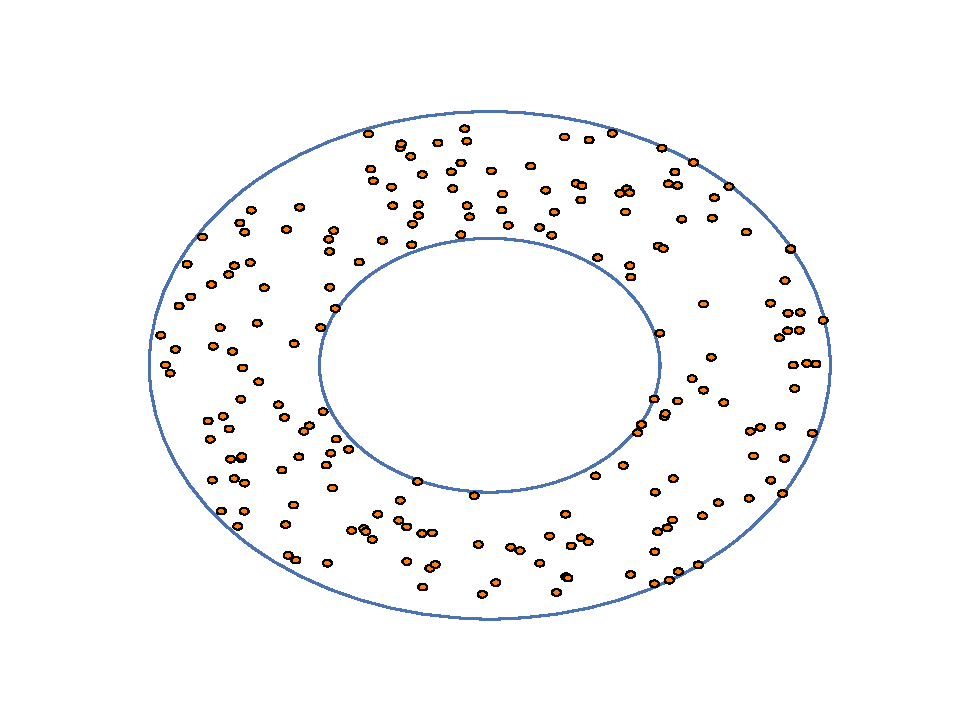
\includegraphics[scale=.45]{annulus.pdf}
    \caption{\label{annulus:points}}
 \end{subfigure}%
  \begin{subfigure}[t]{.5\linewidth}
    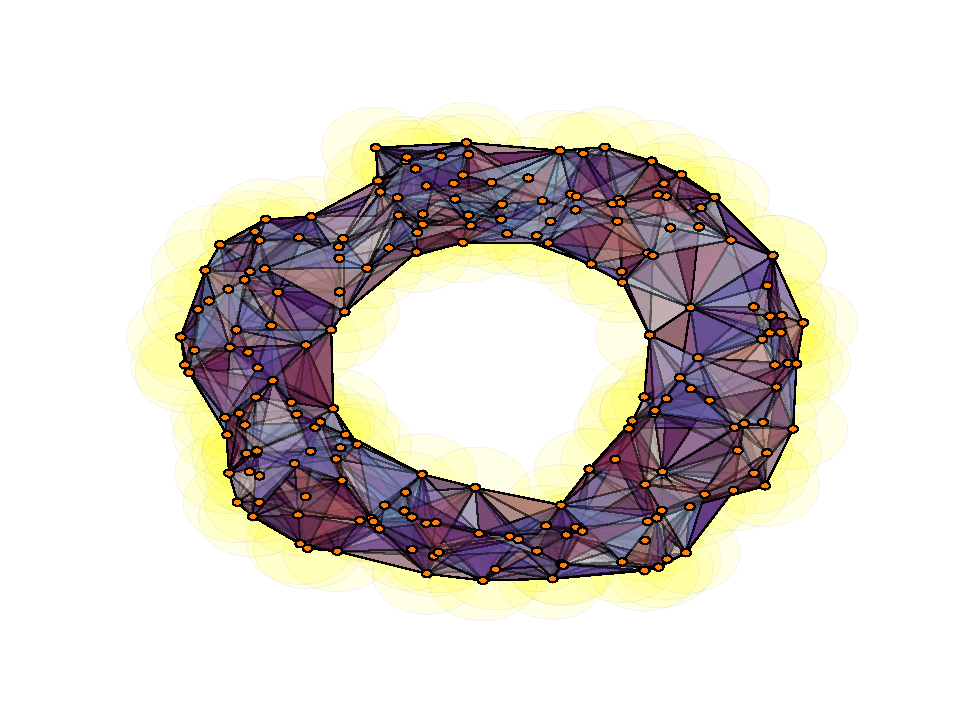
\includegraphics[scale=.45]{annulus_rips.pdf}
    \caption{\label{annulus:imposed}}
 \end{subfigure}
  \caption{\label{annulus} Imposing a simplicial complex \textbf{(b)} on data sampled from an annulus \textbf{(a)}.}
\end{figure}

If we were ignorant of the fact that the underlying space has a the shape of an annulus, which is the situation we more often than not would have in a real-world scenario, being able to deduce the topological properties of this space would tell us that data only lies around a hole. This is where persistent homology comes in, a way of approximating the homology of a space without anything other than the data itself.

The basic principle is quite simple. Using the theory of simplicial homology we can impose a simplicial complex on our dataset as in Figure \ref{annulus:imposed}. A natural way of doing this is defining some form of measure of distance on our data-set, such that when samples are sufficiently close to each other we say they belong to the same simplex.

However, there is a problem with the idea in its naive form. How large is ``sufficiently close''? If we use too large of a distance we end up with all points in a single simplex and retrieve no valuable homological information. On the other hand, if the distance is too small we end up with a simplicial complex with very few connections between vertices and this too could prove uninformative. As we will see, persistent homology circumvents this problem by simply considering \textit{all} possible distances and encoding the homology of the resulting simplicial complexes in a single mathematical object.
% First we need to recall the definition of a homotopy. A homotopy between to continuous maps $f,g$ is another continous map $H: X \times [0,1] \to Y$ such that $H(-,0) = f$ and $H(-,1) = g$. This defines an equivalence relation and we say that $f \simeq g$ meaning that $f$ is homotopy equivalent to $g$.

% We say two topological spaces $X,Y$ are homotopy equivalent, and hence overloading the meaning of this expression, when there exists continuous maps $f: X \to Y$ and $g: Y \to X$ such that $g \circ f \simeq id_{X}$  and $f \circ g \simeq id_{Y}$. This gives an equivalence relation on topological spaces and we write $X \simeq Y$ to mean that they have the same homotopy type.

% After this brief detour we can now look at nerves. We define the nerve of a finite collection of sets to be
% \[nrv(K) = \{ X \subseteq K \mid \bigcap X \neq \emptyset \}\]

% Nerve theorem. Let $F$ be a finite collection of closed convex sets in Euclidean space. Then the nerve of F and the union of the sets in F have the same homotopy type.

\section{Endowing a space with a complex}
A data-set can often be considered as a set of points in Euclidean space. A natural way of endowing a space of points in $\mathbb{R}^{n}$ with a simplicial structure is the following construction.
\begin{definition}[{\cite[p. ~72]{edels}}]
For a family of points $X=\{x_{\alpha}\}_{\alpha}$ in some Euclidean space $\mathbb{R}^{n}$ the \textbf{Čech complex}
$\text{Č}_{\epsilon}$ is given by the abstract simplicial complex whose $k$-simplices are given by a subfamily of $k+1$ points $\{x_{\alpha_{i}}\}$ such that \[\bigcap^{k}_{i=0} B_{\epsilon/2}(x_{\alpha_{i}}) \neq \emptyset\] where $B_{r}(x)$ is the closed ball of radius $r$ centered at $x$.
\end{definition}
The Čech complex is a special case of something called the nerve of a topological space, which guarantees that it has the same homology modules as the union of balls centered at the points \cite[p. ~71]{edels}.

However, the Čech complex is for practical purposes not feasible to compute \cite{ghirst}. The reason being that we need to keep the entire simplicial complex in memory and this can be quite large.

A sort of compromise is the Vietoris-Rips complex as seen in Figure \ref{manyrips}. This complex is a simplification where we do not look for points in common between all balls, but rather say that if $k+1$ have balls that intersect \textit{pairwise} they form a $k$-simplex.

\begin{figure}
  \centering
  \begin{subfigure}[t]{.5\linewidth}
    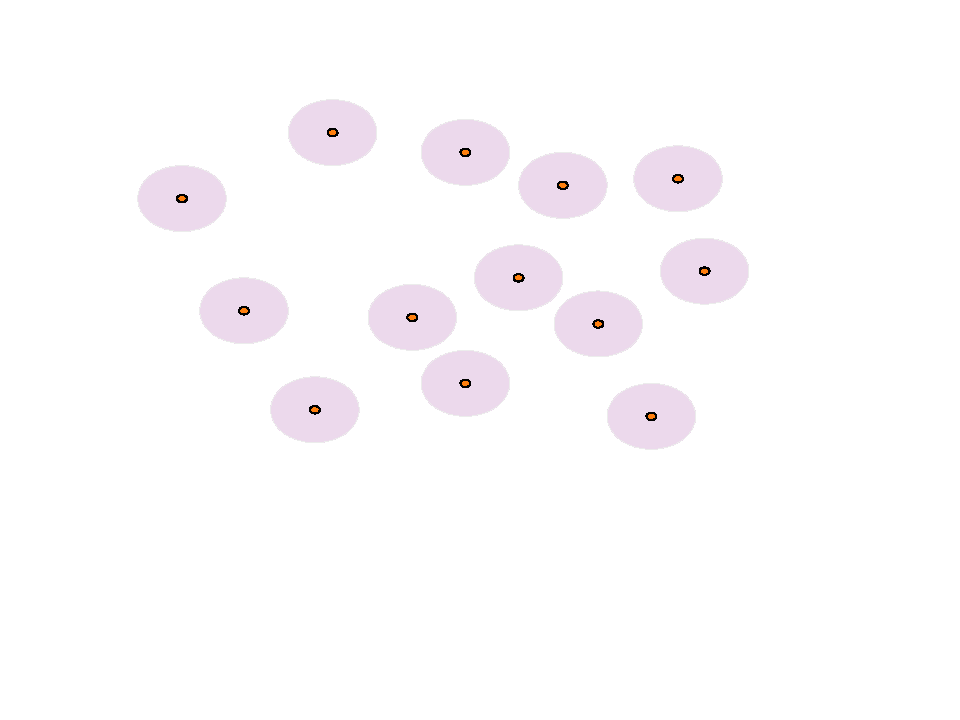
\includegraphics[scale=.5]{rips_eps=01.pdf}
    \caption{$\epsilon=0.1$}
 \end{subfigure}%
  \begin{subfigure}[t]{.5\linewidth}
    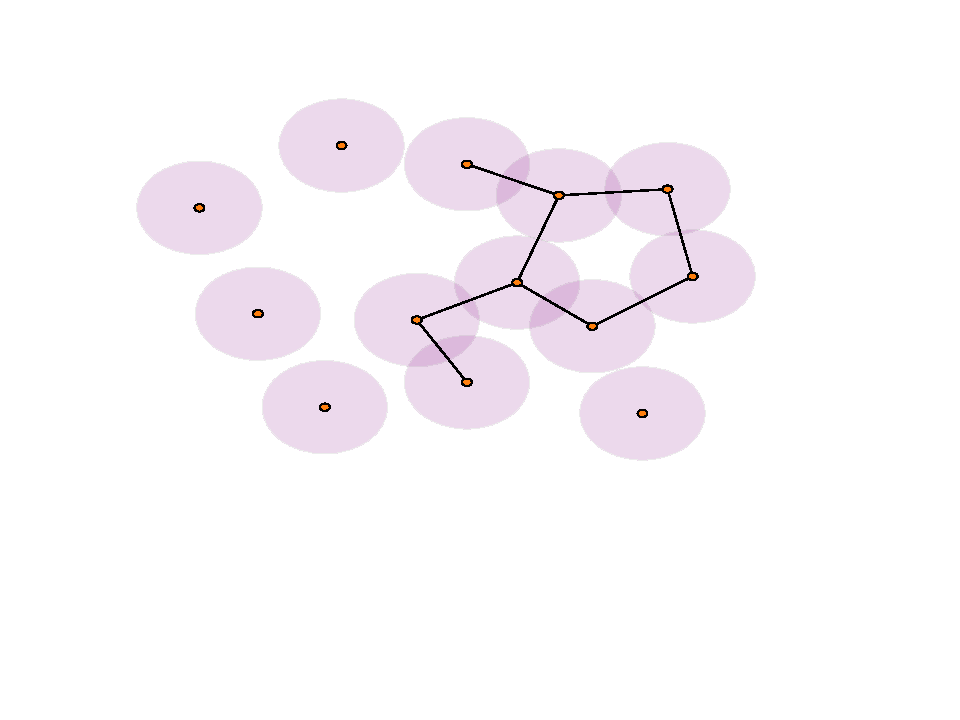
\includegraphics[scale=.5]{rips_eps=015.pdf}
    \caption{$\epsilon=0.15$}
 \end{subfigure}
  \begin{subfigure}[b]{.49\linewidth}
    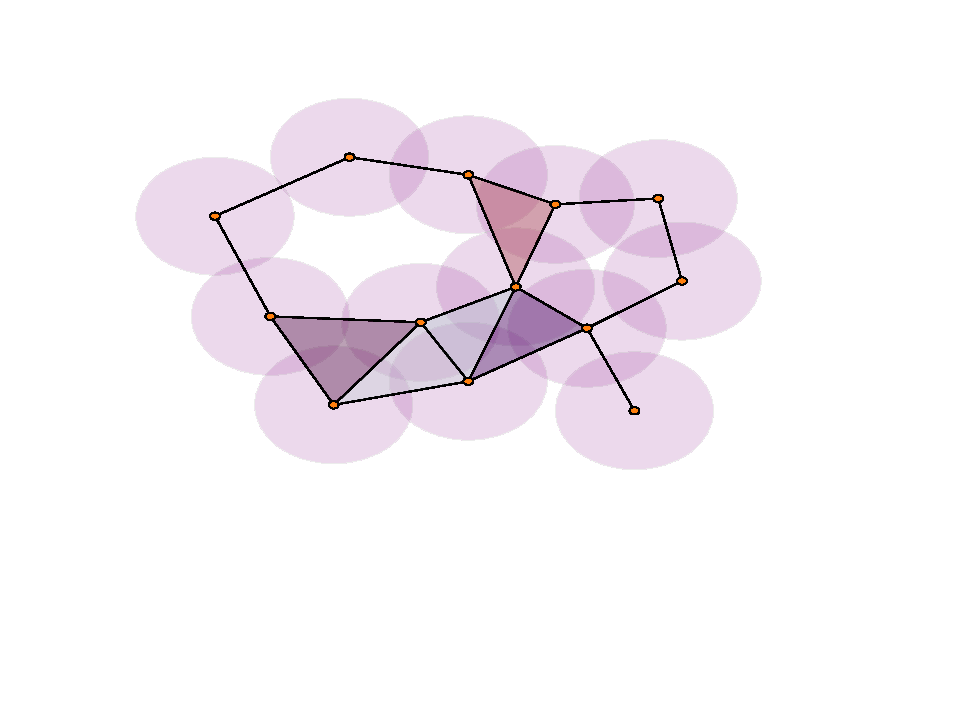
\includegraphics[scale=.5]{rips_eps=02.pdf}
    \caption{$\epsilon=0.2$}
 \end{subfigure}
  \begin{subfigure}[b]{.5\linewidth}
    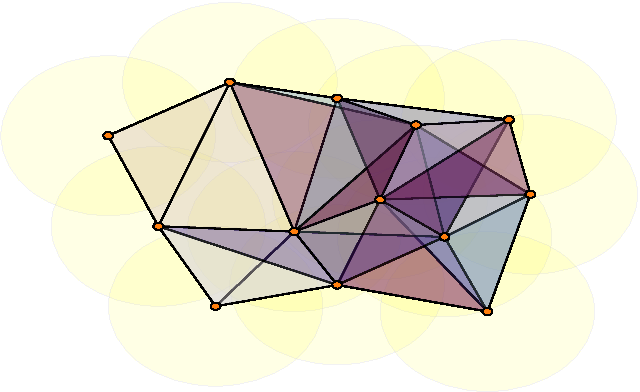
\includegraphics[scale=.5]{rips_eps=03.pdf}
    \caption{$\epsilon=0.3$}
 \end{subfigure}
 \caption{The Vietoris-Rips complex at different $\epsilon$-values.}
 \label{manyrips}
\end{figure}
% \begin{definition}[Vietoris-Rips complex]
% For a given selection of points $\{x_{\alpha}\}$ in some Euclidean space $\mathbb{R}^{n}$ the Vietoris-Rips complex $R_{\epsilon}$ is the abstract simplicial complex whose $k$-simplices are given by $k+1$ points which are pairwise at most $\epsilon$ apart.
% \end{definition}

\begin{definition}[{\cite[p. ~74]{edels}}]
For a family of points $X=\{x_{\alpha}\}_{\alpha}$ in some Euclidean space $\mathbb{R}^{n}$ the \textbf{Vietoris-Rips complex}
$\text{R}_{\epsilon}$ is given by the abstract simplicial complex whose $k$-simplices are given by a subfamily of $k+1$ points $\{x_{\alpha_{i}}\}$ such that for any two points in the collection $x_{\alpha_{i}}, x_{\alpha_{j}}$ we have that \[B_{\epsilon/2}(x_{\alpha_{i}}) \cap B_{\epsilon/2}(x_{\alpha_{j}}) \neq \emptyset\] where $B_{r}(x)$ is the closed ball of radius $r$ centered at $x$.
\end{definition}

The Vietoris-Rips complex does not come with the same guarantee of fidelity to the underlying space as the Čech complex does. However, it is entirely defined by the vertices and the edges of the simplicial complex, allowing it to be stored as a graph.

Given a monotonically increasing sequence of real numbers $(\epsilon_{i})^{n}_{i}$ we can for each $\epsilon_{i}$ associate to a finite set of points $X$ the Vietoris-Rips complex $R_{\epsilon_{i}}$. Then as illustrated in Figure \ref{manyrips} we have inclusions
\begin{center}
\begin{tikzcd}
R_{\epsilon_1} \arrow[hookrightarrow]{r}{\iota} & R_{\epsilon_2} \arrow[hookrightarrow]{r}{\iota} & \dots \arrow[hookrightarrow]{r}{\iota} & R_{\epsilon_{n-1}} \arrow[hookrightarrow]{r}{\iota} & R_{\epsilon_n}.
\end{tikzcd}
\end{center}
For $i<j$ the inclusion $\iota: R_{\epsilon_i} \to R_{\epsilon_{j}}$ induces a map $\iota_{*}: H_{k}(R_{\epsilon_{i}}) \to H_{k}(R_{\epsilon_j})$ and the image of this map tell us which equivalence classes in $H_{k}$ survive when going from $R_{\epsilon_{i}}$ to $R_{\epsilon_{j}}$, in other words the homological features that persist going from resolution $\epsilon_{i}$ to resolution $\epsilon_{j}$ in the Vietoris-Rips construction. The following result then lends some credibility to the Vietoris-Rips complex through its relationship with the Čech complex.
\begin{lemma}[{\cite[Vietoris-Rips Lemma, p. ~74]{edels}}]
  Given $\epsilon > 0$ there is a chain of inclusions
  \[R_{\epsilon} \hookrightarrow C_{\epsilon \sqrt{2}} \hookrightarrow R_{\epsilon \sqrt{2}}\]
\end{lemma}
Hence, any cycle that persists through the induced map $H_{k}(R_{\epsilon}) \to H_{k}(R_{\epsilon'})$ for $\epsilon'  \geq \sqrt{2} \epsilon$ is also present in the Čech complex $\text{Č}_{\epsilon'}$.

The insight that the homological features that persist tell us more than the individual homology groups themselves are central to the idea of persistent homology. Before we give the formal definition of persistent homology we must first generalize the concept of endowing a space with a complex.

\begin{definition}
A \textbf{filtration} $F$ of a simplicial (or cubical) complex $K$ is a totally ordered set of subcomplexes $K^{i}  \subseteq K$ for $i \in \mathbb{N}$ such that if $i \leq j$ then $K^{i} \subseteq K^{j}$.
\end{definition}

Note that the Čech and Vietoris-Rips constructions over a sequence of resolutions are two instances of filtrations, but with this definition we are not restricted to them alone. With this definition in place, we can state the formal definition of persistent homology.

\begin{definition}\label{phfirstdef}
  For $p > 0$ the \textbf{$p$-persistent $k$th homology module} of filtration $F$ is given as
  \[H^{i,p}_{k} = Z^{i}_{k}/(B^{{i+p}}_{k} \cap Z^{i}_{k})\]
  where $Z^{i}_{k},B^{i}_{k}$ are the cycle and boundary modules of the resulting chain complexes $C_*(F_{i})$
\end{definition}
This module is well-defined since the inclusion $K^{i} \hookrightarrow K^{i+p}$ induces inclusions $C^{i}_{k} \hookrightarrow C_{k}^{i+p}$ hence we have inclusions $Z^{i}_{k} \hookrightarrow C^{i}_{k} \hookrightarrow C_{k}^{i+p}$ and so $Z^{i}_{k}$ is a submodule of $C^{i+p}_{k}$. Furthermore, it captures precisely what we have been alluding to earlier: the $p$ persistent homology modules are exactly the equivalence classes that survive up to some filtration $p$.


\section{Persistence Module}
While Definition \ref{phfirstdef} serves as a sufficient framework for persistent homology, it is still particular in the sense that it is stated in terms of filtrations and chain complexes arising from them. It is possible to make the notion of persistence even more general which allows us to understand its algebraic structure. This does not mean that we should entirely discard our anchoring of persistent homology in the realm of simplicial complexes, as it relates closely to how we will do persistent homology in practice, but rather we should let this more abstract approach serve as the theoretical underpinning which opens up the possibility of other types of approximation of data than simplicial complexes.

\begin{definition}[{\cite[p. ~2]{weibel1994}}]
  Let $C_{*},D_{*}$ be chain complexes over some ring $R$. A \textbf{chain map} $u: C_{*} \to D_{*}$ is a family of $R$-module homomorphisms $u_{k}: C_{k} \to D_{k}$ such that the following diagram commutes
  \begin{center}
% https://tikzcd.yichuanshen.de/#N4Igdg9gJgpgziAXAbVABwnAlgFyxMJZARgBoAGAXVJADcBDAGwFcYkQBhAfWAGsBqYgF8QQ0uky58hFACYK1Ok1btuvUeJAZseAkQDMCmgxZtEnHrwC0wjRJ3SiZYopMrzAEUuCRY+1L05UhdjZTMQL3U-LUldGWRDEKVTdi8+G19NbQD48iNk9xAAHSKoCBwEaOy4ojykt3CSsoq7GIdA5AAWfIb2JvLKrNjHFG76sL7SgdFFGCgAc3giUAAzACcIAFskADYaHAgkPILGorR6Nbwmb1lM1Y3txGODpEMT9mZvW2j1raQAdn2h0Qb165hK50uWGufH4t1av0ez2BZHe4LOFyujC+dxAiKQqJeiHkaOKGKhMN4uPxIKBSG6pIhmOh2Nh300NIZRIArKEUujIViuFEOQ8kCSeXzCp90uz7n9iXTEAAOKWnQUsywZBFixC8kBEgCcasmGsp2p+usJwIZYJAnyilCEQA
\begin{tikzcd}
\dots \arrow[r, "\partial_{k+2}"] & C_{k+1} \arrow[d, "u_{k+1}"] \arrow[r, "\partial_{k+1}"] & C_k \arrow[r, "\partial_{k}"] \arrow[d, "u_k"] & C_{k-1} \arrow[d, "u_{k-1}"] \arrow[r, "\partial_{k-1}"] & \dots \\
\dots \arrow[r, "\partial_{k+2}"] & D_{k+1} \arrow[r, "\partial_{k+1}"]                      & D_k \arrow[r, "\partial_k"]                    & D_{k-1} \arrow[r, "\partial_{k-1}"]                      & \dots
\end{tikzcd}
  \end{center}
\end{definition}

\begin{definition}
  A \textbf{persistence complex} is a family of chain complexes $C^{i}_{*}$ together with chain maps $\iota^{i}: C^{i} \to C^{i+1}$ that go between them in the following way
% https://tikzcd.yichuanshen.de/#N4Igdg9gJgpgziAXAbVABwnAlgFyxMJZARgBpiBdUkANwEMAbAVxiRAGkA9YLAXwH1gAawDUxXiF6l0mXPkIoyAJiq1GLNlyyChEqTOx4CRJeVX1mrRB25YxA4fcnSQGQ-JOkV1Cxutceex09Fzc5YxQABjMfdSsQAB0EqAgcBH1XWSMFZGjvNUs2JJS05wNwnLJI8ziihJoS9NCsjxRTatjC6ySG1Kby7KIAZhiCv0TkvrLM9wjkEfzfeOKpjLDBxVIhmq6J3tK1lrnTbc7xnsbJVRgoAHN4IlAAMwAnCABbJDIQHAgkEZ+dCwDDYAAsIBAhCAzssEvgcHR+Fhpq8Pkhoj8-ohvgw6AAjGAMAAKRwUIAYMCeOGhY1haDoLzwjB0TgyqM+iFMmP+MLq9MZWGZjnEKLeHIxvyQXIRwLBEKh1FxBOJpLYFKpNKWdXhdE4yLZYqQABZqJLEBKgSDrODIZrat04alETwALQig1oxAAVlNWO+MqtIBtCtp2qdgiwbpCz0NnN9SAAHKbLXLbbyHTqI6yXOyedzEABOZOy63yu27JKZwLunOxgBs8fN6Ym-KZDBZSmjIFziAA7I2uVqHa3Be3HJ3RZ7-X6MUOWwy2-woR6OQCzcRvnOkiPmcuKLwgA
\begin{center}
\begin{tikzcd}
                                     & \vdots \arrow[d, "\partial_{k+2}"]                                 & \vdots \arrow[d, "\partial_{k+2}"]                                       &       \\
\dots \arrow[r, "\iota^{i-1}", hook] & C^{i}_{k+1} \arrow[d, "\partial_{k+1}"] \arrow[r, "\iota^i", hook] & C^{i+1}_{k+1} \arrow[d, "\partial_{k+1}"] \arrow[r, "\iota^{i+1}", hook] & \dots \\
\dots \arrow[r, "\iota^{i-1}", hook] & C^i_{k} \arrow[r, "\iota^i", hook] \arrow[d, "\partial_k"]         & C^{i+1}_{k} \arrow[r, "\iota^{i+1}", hook] \arrow[d, "\partial_k"]       & \dots \\
                                     & \vdots                                                             & \vdots                                                                   &
\end{tikzcd}
\end{center}
\end{definition}

% \begin{definition}
% Given a persistence complex we define the $(i,j)$-persistent homology $H_{*}^{{i\to j}}(C)$, where $i < j$, to be the image of the induced homomorphism on homology $\iota_{*}: H_{*}(C_{*}^{i}) \to H_{*}(C_{*}^{j})$.
% \end{definition}
\begin{definition}[\cite{Zomorodian2005}]
  A \textbf{persistence module} $M$ is a family of $R$-modules $M^{k}$ together with module homomorphisms $\phi: M^{k} \to M^{k+1}$.
\end{definition}
With the definition of the persistence module we arrive at an alternate definition of persistent homology, the persistent homology of a persistence complex.
\begin{definition}\label{altdef} For $p>0$ the $p$-persistent homology of a persistence complex $(C_{*}, \iota)$ is denoted $H^{p}_{*}$ and is defined to be the images of the induced homomorphisms $\iota^{p-1}_{*} \circ \iota^{p-2}_{*} \circ \dots \circ \iota^{i}_{*}: H_{*}(C_{*}^{i}) \to H_{*}(C^{p}_{*})$.
\end{definition}
In the light of this definition, we see that the $p$-persistent homology of a persistence complex is a persistence module where the module homomorphisms $\phi$ are the maps induced by the chain maps $\iota: C^{i}_{*} \to C_{*}^{i+1}$. The objects given in definitions \ref{phfirstdef} and \ref{altdef} are in fact isomorphic.
\begin{lemma}
Let $\iota^{i,p}_k: H^{i}_{k} \to H^{p}_{k}$ be the module homomorphism that takes a class in $H^{i}$ to the class which contains that class in $H^{p}$. Then $Im (\iota^{i,p}_{k}) \simeq H^{p}_{k}$.
\end{lemma}
\begin{proof}
  Note that the kernel of $\iota^{{i,p}}$ are exactly those classes of cycles which become boundaries at some index $i,i+1,\dots,p$, hence $\ker (\iota^{i,p}) = (B^{i+p} \cap Z^{i})$. So by the first isomorphism theorem for modules we get that
  \[ Im (\iota^{i,p}) \simeq H^{i}_{k} / \ker(\iota^{i,p}) \simeq H^{i}_{k} / (B^{i+p} \cap Z_{k}^{i}) \simeq (Z^{i}_{k}/B^{i}_{k})/(B^{i+p}_{k}\cap Z^{i}_{k}) \simeq H^{i,p}_{k} \]
  where last isomorphism follows from the fact that $B^{i}_{k} \subseteq B_{k}^{i+p} \cap Z^{i}_{k}$.
\end{proof}

\begin{definition}[\cite{Zomorodian2005}]
We say a persistence module $(M^{k}, \phi^{k})$ is of \textbf{finite type} if each component $M^{k}$ is a finitely generated $R$-module and the maps $\phi^{k}$ are isomorphisms for $k > N$ for some integer $N$.
\end{definition}

When we start with a finite simplicial complex $K$ we get that $C_{*}(K)$ consists of finitely generated $R$-modules since the number of simplices in each dimension is finite, hence the resulting persistence complex and persistence modules are of finite type.

The most important theoretic result is just around the corner, but before that we need to recall some definitions regarding graded rings and modules.

\begin{definition}
  Let $R$ be a ring. We say $R$ is a \textbf{graded ring} if it can be decomposed as
  \[ R = \bigoplus_{i} R_{i}\]
\end{definition}
Note that given a ring $R$ the polynomial ring $R[x]$ is always a graded ring, since it can be decomposed into $R[x] = Rx^{0} \oplus Rx^{1} \oplus \dots$

\begin{definition}
A non-zero element $r$ in a graded ring $R$ is said to be homogeneous of degree $n$ if $r \in R_{n}$ and $r \not \in R_{j}$ for all $j \neq n$.
\end{definition}

In other words, the homogeneous elements of a graded ring are those elements that are contained to a single component. Adding elements from different components give us elements that are not homogeneous.
\begin{definition}
  Let $R = \bigoplus_{{i}} R_{i}$ be a graded ring and $M$ an $R$-module. We say that $M$ is a \textbf{graded $R$-module} if $M$ decomposes as
  \[M = \bigoplus_{i} M_{i} \]
  where $M_{i}$ are submodules of $M$, such that $R_{i}M_{j} \subseteq M_{i+j}$.
\end{definition}

Most of the ordinary algebraic constructions on modules hold for graded modules as well. The only additional requirement is that they preserve homogeneous elements in the obvious way. For example, a morphism of graded modules is a morphism of modules such that it preserves degree. In other words, a morphism takes an element in a graded module of degree $n$ to an element in another graded module of degree $n$. Similarly, a graded submodule of a module is simply a graded module such that each component is a submodule of the corresponding component in the parent module.

We can now see that if we have a persistence module $M$ over some ring $R$ and we give $R$ a graded structure by considering $R[t]$ then a graded module structure on $M$ is given by
\[ \alpha(M) = \bigoplus^{\infty}_{k=0} M^{k}\]
The action $t^{p}$ sends $M^{k} \to M^{k+p}$ by $p$ repeated applications of $t$, in other words $t$ shifts the elements up in the graduation by its power
\[ t \cdot (m^{0}, m^{1}, m^{2}, \dots  ) = (0, \phi^{0}(m^{0}), \phi^{1}(m^{1}),\phi^{2}(m^{2}),\dots) \]
and so we get that $R[t]_{p}M^{k} = Rt^{p}M^{k} \subseteq M^{k+p}$ which satisfies the condition we gave in our definition of a graded module.

The map $\alpha$ is actually a functor between the category of persistence modules and graded modules \cite{ghirst} which becomes an isomorphism of categories when considering persistence modules of finite type over a field. Hence, for ease of notation we will simply consider a persistence module to be a graded module when the aforementioned conditions are fulfilled. This gives us a lot for free: we do not have to be afraid of taking quotients or direct sums of persistence modules as we know what objects they correspond to in the category of graded modules. For example, we write $H$ for the direct sum of the persistence modules $H_{k}$ and similarly we write $C$ for the persistence complex given by the sum of the persistence modules $C_{k}$.

We now arrive at the result which fully characterizes the algebraic structure of persistent homology. This result sadly comes with the restriction that makes $\alpha$ an isomorphism of categories, namely that it only characterizes persistence modules of finite type over a field. The more general problem is under the functor $\alpha$ equivalent to characterizing graded $R[t]$ modules over an arbitrary ring $R$, which is known to be a hard problem \cite{ghirst}.
\begin{theorem}[{\cite{Zomorodian2005}}] \label{structurethm1}
  For a persistence module $M$ of \textit{finite type} over a field $\mathbb{F}$,
  \[M \cong \bigoplus_{i} t^{p_{i}} \cdot \mathbb{F}[t] \oplus (\bigoplus_{j} (t^{r_{j}} \cdot \mathbb{F}[t]) / (t^{s_{j}}) \]

\end{theorem}

While the restriction to a field $\mathbb{F}$ somewhat limits the usefulness of the decomposition, we often in practice prefer working in $\mathbb{Z}_{2}$ due to computational aspects and hence in most cases it poses no real problem.

The proof of Theorem \ref{structurethm1} is constructive and ultimately leads to an algorithm for computing persistent homology in terms of linear algebra. Hence, persistent homology is computable in practical applications even for large data-sets. Due to the intimate relation between the proof and the computational aspects we will give it an appropriate treatment in the next section.

Theorem \ref{structurethm1} has an intuitive explanation in terms of filtrations: when $M$ is the persistent homology $H$ given by some filtration $F$, the free part consists of generators which appear in the subcomplex $F_{p_{i}}$ and continue to exist for all future filtrations. The torsional part consists of generators which appear at in the subcomplex $F_{r_{j}}$ and disappear in  $F_{r_{j}+s_{j}}$. Furthermore, the decomposition provides the $p$-persistent homology for all $p$ and so we circumvent the problem of having to choose an optimal step of the filtration of which to compute homology.

We can make this association of the decomposition of a persistence module with intervals more precise through the following definitions.

\begin{definition}
  For a persistence module $M$ as in Theorem \ref{structurethm1} we associate the interval $(i,j) \in \mathbb{N}\cup \{\infty\}$ to ${M}$ as
  \[Q(i,j):= t^{i} \cdot \mathbb{F}[t]/t^{{j-i}},\]

  \[Q(i,\infty):= t^{i} \cdot \mathbb{F}[t].\]
  Furthermore, given a multiset of intervals $S = \{(i_{0},j_{0}),\dots,(i_{n},j_{n})\}$ we say that
  \[Q(S) := \bigoplus_{k} Q(i_{k},j_{k}).\]
  The \textbf{barcode} $\mathbf{B_{M}}$ is the multiset of intervals $Q^{-1}(M)$.
\end{definition}


In the obvious way, $Q$ is a bijection which maps each summand in the decomposition of a persistence module to an interval. This gives us a correspondence between infinite intervals and generators of the free part and finite intervals and generators of the torsional part.


\section{Proof of the Structure Theorem}
As promised we will now derive the connection between linear algebra and persistence modules. For this part we will abuse the isomorphism of categories between persistence modules and graded modules over $\mathbb{F}[t]$ and readily switch between the two perspectives.  A key observation is that for every (graded) module $M$ there is an exact sequence
\[ K \to G \to M \to 0\]
where $G$ is the free module on the generators of $M$ and $K$ is the free module on the generators of $\ker G \to M$. By the first isomorphism theorem this exact sequence yields an isomorphism $M \cong G/\text{im }(K \to G)$, and hence we can characterize $M$ by only knowing $K,G$ and $f$. We call such a sequence a \textbf{presentation} of $M$.
\begin{lemma}[{\cite[Theorem 7]{skraba}}]
  For a finitely generated graded module $M$ over $\mathbb{F}[t]$ there a presentation of $M$ given by a short exact sequence
  \[ 0 \to K \to G \to M \to 0\]
  where $G,K$ are finitely generated.
\end{lemma}
\begin{proof}
First of all, note that since $G$ is the free module on the generators of $M$ and $M$ has a finite set of generators so does $G$.

A standard result due to Hillbert (see for example \cite[Theorem 4, p. ~76]{Cox+Others/1991/Ideals}) is that any submodule of a finitely generated module over $\mathbb{F}[t]$ is finitely generated. This means in particular that $\ker (G \to M)$ is finitely generated, as it is a submodule of $G$ over $\mathbb{F}[t]$.

We start by proving that $\ker (G \to M)$ is free. Suppose for contradiction that $\ker (G \to M)$ is not free, then for a finite set of generators $\{k_{i}\}^{n}_{i=0}$ of $\ker (G \to M)$ the assumption implies linear dependence such that
\[\sum_{i} r_{i}t^{a_{i}}k_{i}=0  \iff t^{b} \sum_{i} r_{i}t^{a_{i}-b}k_{i} = 0 \implies \sum_{i} r_{i}t^{a_{i}-b}k_{i} = 0 \]
where $b = \min\{a_{i} \mid r_{i} \neq 0\}, r_{i} \in \mathbb{F}$ and the last implication follows from that $\ker(G \to M)$ is a submodule of the free module $G$. Then for some term in the sum we have that $a_{j}=b$ and $ k_{j} \neq 0 $ which gives us that
\[
  r_{j}t^{a_{j}-b}k_{j}=r_{j}k_{j} \implies k_{j} = - r_{j}^{-1}\sum_{i \neq j} r_{i}t^{a_{i}-b}k_{i}.
\]
But then $k_{j}$ can be given as a linear sum of generators of $\ker (G \to M)$ so it can be excluded from the list of generators. Iterating the argument above then exhausts the finite set of generators until the set consists of linear independent generators, hence $\ker (G \to M)$ is free.

Since $\ker (G \to M) = \text{im } (K \to G)$ by the exactness of the presentation and $K$ is the free module on the generators of this finitely generated, free image it follows that $K \cong \text{im } K \to G$ and so $K \to G$ is injective and $K$ is finitely generated.
\end{proof}
When $K,G$ are free and finitely generated the presentation yields a map $\mathbb{F}[t]^{n} \to \mathbb{F}[t]^{m}$, in other words it can for a given choice of bases be represented by a matrix in $\mathbb{F}[t]^{n \times m}$ which we call a \textbf{presentation matrix} of $M$. This is the vital connection between persistence modules and linear algebra. By reducing this matrix, much like in the process of Gaussian elimination, we end up with a matrix that describes compatible bases in $K$ and $G$. Then $M$ is generated by the basis in $G$ with relations given by the basis in $K$.

\begin{definition}
A matrix with coefficients in $\mathbb{F}[t]$ is in \textbf{graded Smith normal} if its only non-zero entries are on the (possibly permuted) diagonal and these entries are homogeneous elements.
\end{definition}

We will now describe an algorithm for computing the graded Smith normal form. Since the resulting matrix will consist of linearly independent columns and rows they define a basis for the column and row space.
\clearpage
\begin{algorithm}[h]
\caption{Reduction to graded Smith normal form \cite{skraba, Zomorodian2005}}\label{smith}
\begin{algorithmic}[1]
  \State \textbf{Input:} Matrix $ \in \mathbb{F}[t]^{n \times m}$ with homogeneous entries with columns and rows sorted in order of ascending degree.
  \State \textbf{Returns:} Matrix $ \in \mathbb{F}[t]^{n \times m}$ in graded Smith normal form with columns and rows sorted in order of ascending degree.
  \For{$i < m, j < n$}
  \State Eliminate all entries \textit{rightwards} by column additions in row $i$.
  \State Eliminate all entries \textit{upwards} by row additions in column $j$.
  \EndFor
\end{algorithmic}
\end{algorithm}

\begin{proof}(\textbf{Correctness of Algorithm 1.})
  To show the correctness of the algorithm it suffices to show that we can eliminate entries and that such elimination does not change the degrees of the homogeneous basis elements given by the rows and columns. Since columns and rows are finite, we will eventually terminate.

  Suppose we wish to eliminate some entry in row $j$ with an element in row $i$. This implies that $ i > j$ by the algorithm itself. Let the entries be denoted $a_{i}= c \cdot t^{r_{i}}$ and $b_{j} = d \cdot t^{s_{j}}$ respectively. Since the columns and rows are chosen to be homogeneous, we know that they can be written this way. The matrix is sorted in ascending degree order in both rows and columns, which implies that $\deg(a_{i}) \leq \deg(b_{j})$, hence we can always eliminate $b_{j}$ by adding $t^{s_{j}-r_{i}} \frac{-d}{c} \cdot a_{i}$. Furthermore, if $\gamma_{i},\gamma_{j}$ are the basis elements of rows $i,j$ then we know from linear algebra that the addition causes a change of basis $\gamma'_{i}:=\gamma_{i}-t^{s_{j}-r_{i}} \frac{-d}{c} \cdot \gamma_{j}$. We get that $\deg(\gamma'_{i})=\max\{\deg(\gamma_{i}), (s_{j}-r_{i}+\deg(\gamma_{j})\}$, but since $a_{i},b_{j}$ are entries of the same homogeneous column this implies that $r_{i} + \deg(\gamma_{i}) = s_{j} + \deg(\gamma_{j})$, hence $\deg(\gamma'_{i}) = \deg(\gamma_{i})$. An identical argument holds for if we wish to eliminate by column additions, with the exception that it is $\gamma_{j}$ that changes basis.
\end{proof}
When a presentation matrix of $M$ is put into graded Smith normal form by Algorithm 1 it gives us compatible bases for $K$ and $G$ and the isomorphism becomes \[M\cong \frac{\text{basis  elements given by rows  }}{\text{basis elements given by non-zero rows times their entry}}\]
To understand how we can intrepret the presentation matrix as such, consider that the rows give a basis for $G$ under the inclusion $K \hookrightarrow G$. The non-zero rows tell us which of those basis elements become basis elements of $K$ when multiplied by their corresponding non-zero entry and thus define when they are killed in $M$.

We are now ready to prove \textbf{Theorem \ref{structurethm1}}.

\begin{proof}
  The module $M$ is of finite type so it has a presentation matrix $P$. By reducing $P$ to graded Smith normal form with Algorithm 1 we get a matrix $P'$. Since $M \cong G/K$ by the first isomorphism theorem we have that free part of $M$ is given by the basis elements of $G$ associated with the zero rows of $P'$, as these are basis elements which are not hit by the inclusion $K \hookrightarrow G$ in any part of the grading. Furthermore, the torsional part in the decomposition is given by the non-zero rows which define basis elements of $G$ that when shifted by their entry are basis elements of $K$ and thus are killed in $M$. This proves the existence of the decomposition.

  What remains to show is that the decomposition is unique no matter our choice of basis for $G$ and $K$. This actually follows from a much more general result, the Krull-Schmidt Theorem \cite[p. ~115]{jacobson2009basic}, but we will give an elementary proof. Suppose that we have two different decompositions of $M$ that we denote $C,D$. We claim that they are identical up to permutation of components and modulo trivial components. We have homomorphisms
  \[
    f_{ij} := C_{i} \overset{\iota_{C_{i}}}{\hookrightarrow} \overset{\phi}{C \cong M  \cong D}  \overset{\pi_{D_{j}}}{\twoheadrightarrow} D_{j},
  \]
\[
  g_{ij} := D_{j} \overset{\iota_{D_{j}}}{\hookrightarrow} \overset{\phi^{-1}}{D \cong M  \cong C}  \overset{\pi_{C_{i}}}{\twoheadrightarrow} C_{i},
  \]
  % \[
  %   g_{ij} :=  D_{j} \hookrightarrow D \cong M  \cong C  \twoheadrightarrow C_{i}
  % \]
  where the maps are the obvious inclusions and projections from and onto components and the isomorphism through the decomposition of $M$. Then for at least one pair $i,j$ the homomorphism $f_{ij}$ cannot be the zero map since $\bigoplus_{i,j} g_{ij} \circ f_{ij}: C \to C$ is an automorphism of $C$. Assume that $i=1,j=1$, if this is not the case we can just permute the summands.  Then $f_{11}$ (by symmetry all arguments below hold for $g_{ij}$ as well) is an isomorphism $C_{1} \cong D_{1}$ since the graded isomorphism $\bigoplus_{i,j} f_{ij}$ takes a homogeneous element $t^{a} \to c \cdot t^{a}$ for some $c \in \mathbb{F}$.

  Looking at \[f_{2_{+}}:= \bigoplus_{i=2,j=2} f_{ij}: \oplus_{i=2}C_{i} \to \oplus_{j=2} D_{j}\] we can deduce that it is also an isomorphism.

  For injectivity, note that if $\hat c = (c_{2},c_{3},\dots) \in \ker f_{2+}$ then $\phi$ has to map $\oplus_{i=2} \iota_{C_{i}} \hat c=(0,c_{2},c_{3},\dots)$ to $(d_{1},0,0,\dots)$ for some $d_{1} \in D_{1}$ since the final map is just the projections $\oplus_{j=2}\pi_{D_{j}}$. By post-composing $\iota_{C_{1}} \phi^{-1}$ we get

  \[\iota_{D_{1}}(d_{1})= \phi \oplus_{i=2}\iota_{C_{i}}(\hat c) \iff
  \]
  \[
    \pi_{C_{1}} \phi^{-1} \iota_{D_{1}}(d_{1})=  \pi_{C_{1}} \phi^{-1} \phi \oplus_{i=2}\iota_{C_{i}}(\hat c) \iff
      g_{11}(d_{1}) = 0
    \]
    which gives us that $\hat c = 0$. Hence, $f_{2_{+}}$ is injective.

    For surjectivity take any element $\hat d := (d_{2},d_{3},\dots)$ in $\oplus_{j=2}D_{j}$. Since $\phi$ is an isomorphism there exists some $d_{1} \in D_{1}$ such that

    \[\hat c := (0,c_{2},c_{3},\dots) = \phi^{-1}(d_{1},d_{2},d_{3},\dots)\] for some $\hat c \in C$ and so we get
    \[\oplus_{j=2} \pi_{D_{j}} \phi \oplus_{i=2}\iota_{C_{i}} (c_{2},c_{3},\dots) = f_{2+}(c_{2},c_{3},\dots)= \hat d.
      \]
  So we get that $f_{2_{+}}$ is an isomorphism and by symmetry $g_{2+}$ is also an isomorphism. Hence, $g_{2+} f_{2_{+}}$ is an automorphism and we can repeat the same argument to find new indices $i,j$ such that $f_{ij}$ and $g_{ij}$ are isomorphisms. Since the decomposition is a direct sum, there are a finite number of non-trivial modules and so we will eventually have exhausted all of them. The rest of the summands not covered by these isomorphisms must then consist of trivial modules and so we have proven the uniqueness of the decomposition up to permutation and trivial modules.

\end{proof}
Now for explicitly computing persistent homology we have the presentation

\[
  0 \to B \to Z \to H \to 0
\]
and so we could theoretically apply the proof above and get a decomposition of $H$, but this comes with one caveat: to give a presentation matrix of $H$ requires us to first have a basis of $Z$, which we typically do not have. Instead we have the boundary map $\partial: C \to C$ which has as its image $B$ and $Z$ as its kernel. Hence, we must first compute the Smith graded normal form of the map $\partial$ which gives us a compatible basis in both $B$ and $Z$. Then we compute the Smith normal form of the inclusion map $B \to Z$ from which we can derive the barcode $\mathbf{B}_{H}$.

\begin{example}\label{bddreduce}
Consider the filtration given in Figure \ref{filtrationstack}. For simplicity we work in $\mathbb{F}=\mathbb{Z}_{2}$. The persistence complex has basis given by the simplices $v_{0},v_{1},v_{2},v_{12},v_{20},v_{01},v_{03},v_{120}$. We get the following boundaries by evaluating the boundary map $\partial$ on the simplices which generate the chain complex \[v_{2}+v_{1},t(v_{1})+t^{2}(v_{0}),t(v_{2})+t^{2}(v_{0}),v_{3}+t^{2}v_{0}, t^{2}(v_{12})+t(v_{10})+t(v_{20}).\]
Hence we have the following matrix representing the map $\partial$:
\[
  \bordermatrix{
    & v_{0} & v_{1} & v_{2} & v_{3} & v_{12} & v_{20} & v_{01} & v_{03} & v_{120}\cr
    v_{0}  &.&.&.&.&.&t^{2}&t^{2}&t^{2}&.\cr
    v_{1}  &.&.&.&.&1&.&t&.&.\cr
    v_{2}  &.&.&.&.&1&t&.&.&.\cr
    v_{3}  &.&.&.&.&.&.&.&1&.\cr
    v_{12} &.&.&.&.&.&.&.&.&t^{2}\cr
    v_{20} &.&.&.&.&.&.&.&.&t\cr
    v_{01} &.&.&.&.&.&.&.&.&t\cr
    v_{03} &.&.&.&.&.&.&.&.&.\cr
    v_{120}&.&.&.&.&.&.&.&.&.
    }
  \]
  Reducing this matrix to graded Smith normal form while keeping track of basis changes gives us the matrix
%     \[
%       \to
% \bordermatrix{
%     & v_{0} & v_{1} & v_{2} & v_{3} & v_{12}  & v_{20} + tv_{12}& v_{01} & v_{03} & v_{120}\cr
%     v_{0}  &.&.&.&.&.&t^{2}&t^{2}&t^{2}&.\cr
%     v_{1}  &.&.&.&.&1&t&t&.&.\cr
%     v_{2}  &.&.&.&.&1&.&.&.&.\cr
%     v_{3}  &.&.&.&.&.&.&.&1&.\cr
%     v_{12} &.&.&.&.&.&.&.&.&t^{2}\cr
%     v_{20} &.&.&.&.&.&.&.&.&t\cr
%     v_{01} &.&.&.&.&.&.&.&.&t\cr
%     v_{03} &.&.&.&.&.&.&.&.&.\cr
%     v_{120}&.&.&.&.&.&.&.&.&.
%     }
% \]

%     \[
% \bordermatrix{
%     & v_{0} & v_{1} & v_{2} & v_{3} & v_{12} & v_{20}+tv_{12} & v_{01}+v_{20}+tv_{12} & v_{03} & v_{120}\cr
%     v_{0}  &.&.&.&.&.&t^{2}&.&t^{2}&.\cr
%     v_{1}  &.&.&.&.&1&t&.&.&.\cr
%     v_{2}  &.&.&.&.&1&.&.&.&.\cr
%     v_{3}  &.&.&.&.&.&.&.&1&.\cr
%     v_{12} &.&.&.&.&.&.&.&.&t^{2}\cr
%     v_{20} &.&.&.&.&.&.&.&.&t\cr
%     v_{01} &.&.&.&.&.&.&.&.&t\cr
%     v_{03} &.&.&.&.&.&.&.&.&.\cr
%     v_{120}&.&.&.&.&.&.&.&.&.
%     }
%   \]

%     \[
% \bordermatrix{
%     & v_{0} & v_{1} & v_{2} & v_{3} & v_{12} & v_{20}+tv_{12} & v_{01}+v_{20}+tv_{12} & v_{03} & v_{120}\cr
%     v_{0}  &.&.&.&.&.&t^{2}&.&t^{2}&.\cr
%     v_{1}  &.&.&.&.&.&t&.&.&.\cr
%     v_{2}+v_{1}  &.&.&.&.&1&.&.&.&.\cr
%     v_{3}  &.&.&.&.&.&.&.&1&.\cr
%     v_{12} &.&.&.&.&.&.&.&.&t^{2}\cr
%     v_{20} &.&.&.&.&.&.&.&.&t\cr
%     v_{01} &.&.&.&.&.&.&.&.&t\cr
%     v_{03} &.&.&.&.&.&.&.&.&.\cr
%     v_{120}&.&.&.&.&.&.&.&.&.
%     }
%   \]

%     \[
% \bordermatrix{
%     & v_{0} & v_{1} & v_{2} & v_{3} & v_{12} & v_{20}+tv_{12} & v_{01}+v_{20}+tv_{12} & v_{03} & v_{120}\cr
%     v_{0}  &.&.&.&.&.&.&.&t^{2}&.\cr
%     v_{1}+tv_{0}  &.&.&.&.&.&t&.&.&.\cr
%     v_{2}+v_{1}  &.&.&.&.&1&.&.&.&.\cr
%     v_{3}  &.&.&.&.&.&.&.&1&.\cr
%     v_{12} &.&.&.&.&.&.&.&.&t^{2}\cr
%     v_{20} &.&.&.&.&.&.&.&.&t\cr
%     v_{01} &.&.&.&.&.&.&.&.&t\cr
%     v_{03} &.&.&.&.&.&.&.&.&.\cr
%     v_{120}&.&.&.&.&.&.&.&.&.
%     }
%   \]
% \[
% \bordermatrix{
%     & v_{0} & v_{1} & v_{2} & v_{3} & v_{12} & v_{20}+tv_{12} & v_{01}+v_{20}+tv_{12} & v_{03} & v_{120}\cr
%     v_{0}  &.&.&.&.&.&.&.&.&.\cr
%     v_{1}+tv_{0}  &.&.&.&.&.&t&.&.&.\cr
%     v_{2}+v_{1}  &.&.&.&.&1&.&.&.&.\cr
%     v_{3}+t^{2}v_{0}  &.&.&.&.&.&.&.&1&.\cr
%     v_{12} &.&.&.&.&.&.&.&.&t^{2}\cr
%     v_{20} &.&.&.&.&.&.&.&.&t\cr
%     v_{01} &.&.&.&.&.&.&.&.&t\cr
%     v_{03} &.&.&.&.&.&.&.&.&.\cr
%     v_{120}&.&.&.&.&.&.&.&.&.
%     }
%   \]
%     \[
% \bordermatrix{
%     & v_{0} & v_{1} & v_{2} & v_{3} & v_{12} & v_{20}+tv_{12} & v_{01}+v_{20}+tv_{12} & v_{03} & v_{120}\cr
%     v_{0}  &.&.&.&.&.&.&.&.&.\cr
%     v_{1}+tv_{0}  &.&.&.&.&.&t&.&.&.\cr
%     v_{2}+v_{1}  &.&.&.&.&1&.&.&.&.\cr
%     v_{3}+t^{2}v_{0}  &.&.&.&.&.&.&.&1&.\cr
%     v_{12} &.&.&.&.&.&.&.&.&.\cr
%     v_{20} &.&.&.&.&.&.&.&.&t\cr
%     v_{01}+tv_{12} &.&.&.&.&.&.&.&.&t\cr
%     v_{03} &.&.&.&.&.&.&.&.&.\cr
%     v_{120}&.&.&.&.&.&.&.&.&.
%     }
%   \]

    \[
\bordermatrix{
    & v_{0} & v_{1} & v_{2} & v_{3} & v_{12} & v_{20}+tv_{12} & v_{01}+v_{20}+tv_{12} & v_{03} & v_{120}\cr
    v_{0}  &.&.&.&.&.&.&.&.&.\cr
    v_{1}+tv_{0}  &.&.&.&.&.&t&.&.&.\cr
    v_{2}+v_{1}  &.&.&.&.&1&.&.&.&.\cr
    v_{3}+t^{2}v_{0}  &.&.&.&.&.&.&.&1&.\cr
    v_{12} &.&.&.&.&.&.&.&.&.\cr
    v_{20} &.&.&.&.&.&.&.&.&.\cr
    v_{01}+tv_{12}+v_{20} &.&.&.&.&.&.&.&.&t\cr
    v_{03} &.&.&.&.&.&.&.&.&.\cr
    v_{120}&.&.&.&.&.&.&.&.&.
    }
  \]
  From the reduction to normal form we can read off a basis for $Z$ given by the zero columns and the basis of $B$ given by the non-zero rows together with their non-zero entry. This gives us a presentation matrix of $H$ from the inclusion $B \hookrightarrow Z$

  \[
    \bordermatrix{& v_{2}+v_{1} & tv_{1}+t^{2}v_{0} & v_{3}+t^{2}v_{0} & tv_{01}+t^{2}v_{12}+tv_{20} \cr
      v_{0} & . & t^{2} & t^{2} & . \cr
      v_{1} & 1 & t & . & .     \cr
      v_{2} & 1 & . & . & .     \cr
      v_{3} & . & . & 1 & .     \cr
      v_{01}+v_{20}+tv_{12}  & . & . & . & t
      }
  \]

  Reduction of this matrix to Smith normal form gives us
  \[
    \begin{pmatrix}
      . & . & . & . \\
      . & t & . & .     \\
        1 & . & . & .     \\
        . & . & 1 & .     \\
        . & . & . & t
        \end{pmatrix}
  \]
% Cycles are $v_{0},[v_{1}],v_{3},tv_{12}-v_{02}+v_{01}$.
  %Anyway..

 We see that there is one zero row given by $v_{0}$ which gives us the interval $[1,\infty)$. This is because $v_{0}$ is the $0$-cycle in Figure \ref{filtrationstack} that eventually becomes the connected component of the entire simplicial complex, hence it never dies. We additionally have two intervals $[2,3)$ and $[3,4)$ from the rows with $t$ as their entry. The first one is the other connected component given by $v_{1}+v_{2}$ which is born at filtration step $2$ and dies when it becomes part of the single connected component given by $v_{0}$ in filtration step 3. The interval $[3,4)$ corresponds to the triangle without interior at filtration step $3$ which later dies at filtration step $4$ when the triangle is filled in.


\begin{figure}[ht]
  \centering
  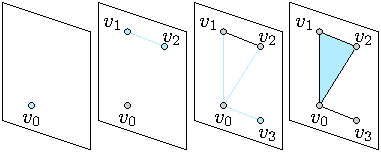
\includegraphics[scale=1.5]{simp_filt.pdf}
  \caption{\label{filtrationstack} Filtration of a simplicial complex showing the intermediate simplicial complex at each filtration step. A blue simplex indicates the simplex was added in that filtration step.}
\end{figure}

% (v_0,v_1,v_2,v_12,v_3,v_20,v_01,v_03,v_120)
% (1,2,2,2,3,3,3,3,4)
\end{example}

Algorithm 1 for a simplicial complex has, just like ordinary Gaussian elimination over fields, worst case time complexity $O(m^{3})$ where $m$ is the  number of simplices \cite{Zomorodian2005}. However, as seen in Example \ref{bddreduce} the boundary matrix is sparse. Furthermore, the decomposition of $H$ can be read entirely from the reduced boundary matrix without constructing an explicit presentation matrix. These are some areas where the algorithm usually is made more efficient, but dwelling on such optimizations is outside the scope of this thesis. For more in-depth treatments on this subject see  \cite{edels} for the theoretical underpinnings and \cite{ripser} for the de facto solution on which many software libraries are based.


\section{Visualizing Persistence}
The persistent homology of a space is not a very easy algebraic object to work with in practical terms. Even when considered under the bijection with intervals it is a multiset of intervals and as such helpful visualizations allow us to analyze and compare persistent homology. There are two principal ways of visualizing the decomposition of a persistence module: barcode diagrams and persistence diagrams.

\subsection{Barcodes}
A \textbf{barcode diagram} is a visual depiction of $\textbf{B}_{H}$ where each bar depicts the start end and end of an interval, or equivalently the birth and death of a particular generator in one of the homology modules.

In Figure \ref{annulus_barcode} we see a barcode diagram generated from points sampled from an annulus. Note that for small values of $\epsilon$ there are many generators of $H_{0}$, this is because the vertices have not been connected into a single component yet.

  We see that there some short intervals appearing for $H_{1}$ at around $\epsilon=0.3$ and we can see that these are not the hole that would represent the annulus, but rather noise that appears before $\epsilon$ has become large enough. At around $\epsilon=0.6$ the simplicial complex now captures the shape of the annulus and indeed the barcode diagram shows that we have one generator of $H_{0}$, the only connected component, and one generator of $H_{1}$ which is the hole in the middle of the annulus.

  Note how this hole in the middle of the annulus is gone when $\epsilon=1$ which highlights that it is difficult to find an optimal $\epsilon$.
\begin{figure}
  \centering
\begin{tikzpicture}
\node[inner sep=0pt] (barcode) at (0,0)
    {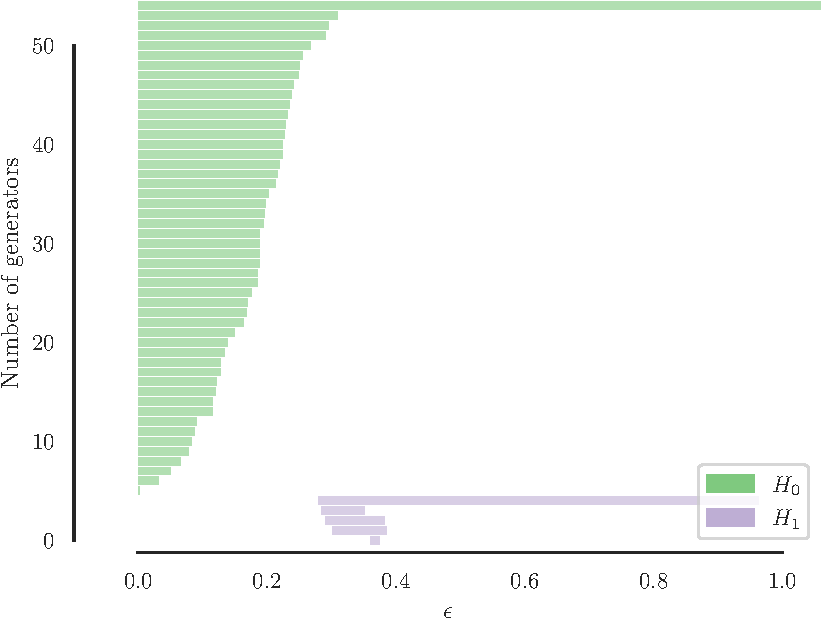
\includegraphics[scale=0.7]{barcode.pdf}};

\node[draw=black!100,line width=0.6mm, inner sep=0pt] (annulus0) at (-3.2,5.1)
    {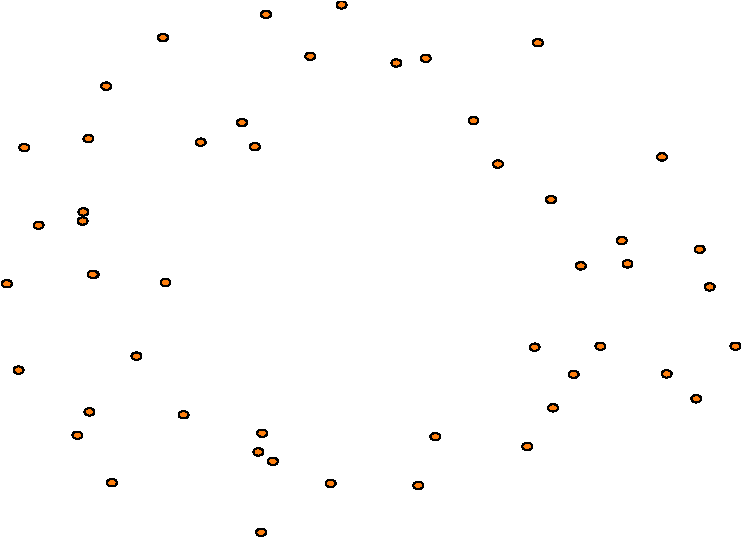
\includegraphics[scale=0.3]{annulus_eps0.pdf}};
    \draw[dotted,thick] (annulus0.south) -- (-3.2,-2.9);

\node[draw=black!100,line width=0.6mm, inner sep=0pt] (annulus3) at (-1,8)
    {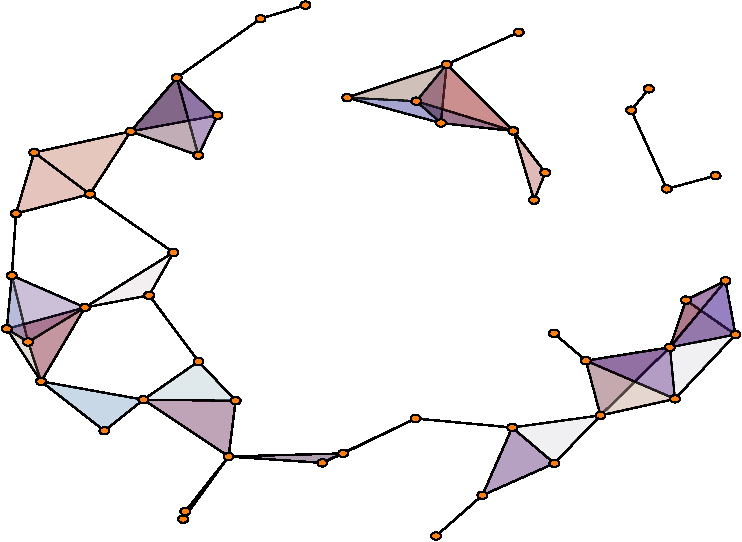
\includegraphics[scale=0.3]{annulus_eps3.pdf}};
\draw[dotted,thick] (annulus3.south) -- (-1,-2.9);

\node[draw=black!100,line width=0.6mm, inner sep=0pt] (annulus5) at (1.2,5.1)
    {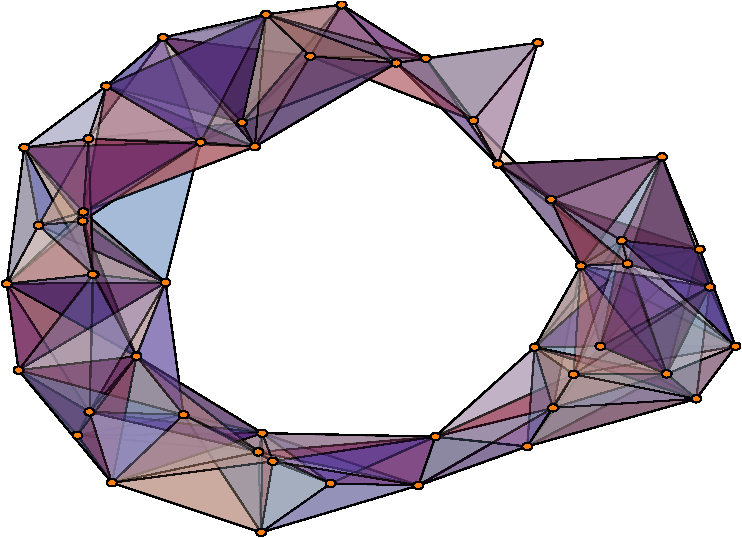
\includegraphics[scale=0.3]{annulus_eps5.pdf}};
    \draw[dotted,thick] (annulus5.south) -- (1.2,-2.9);
\node[draw=black!100,line width=0.6mm, inner sep=0pt] (annulus10) at (4.4,8)
    {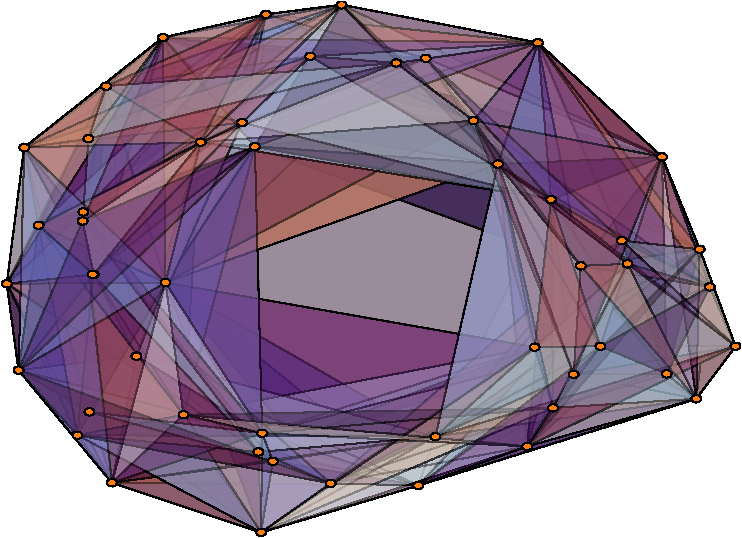
\includegraphics[scale=0.3]{annulus_eps10.pdf}};
\draw[dotted,thick] (annulus10.south) -- (4.4,-1.8);
\draw[dotted,thick] (4.4,-2.74) -- (4.4,-2.9);
\end{tikzpicture}
\caption{\label{annulus_barcode} Persistence barcode showing the birth and death of generators in the homology groups of a Vietoris-Rips complex approximated from points sampled from an annulus at different $\epsilon$. }
\end{figure}
  \subsection{Persistence Diagrams}
  Another way of illustrating persistent homology is the persistence diagram as seen in Figure \ref{pdiagram}.

  \begin{definition}
    The \textbf{persistence diagram} $X$ of a persistence module $M$ is a multiset of points in $\mathbb{R}^{2}\cup \{\infty\}$ defined as
    \[
      X:=\{ (x,y) \in \mathbb{R}^{2} \mid [x,y) \in \mathbf{B}_{M}\} \cup \{ (x,x) \mid | x \in \mathbb{R}\}.
    \]
  \end{definition}
In other words, it is the set of \textit{(birth,death)} pairs given by the intervals associated with the decomposition of $M$ together with all points on the diagonal.

When visualized as in Figure \ref{pdiagram} it serves alternative to the barcode in Figure \ref{annulus_barcode} where we instead plot the $\epsilon$-value on both axes and for each generator we draw a point given by its corresponding interval. When we have a lot of intervals this is a preferable way of visualizing the persistent homology, since unlike the barcode it does not grow vertically with the number of intervals. Generators that never die are mapped at a line representing infinity.

Just like in the barcode in Figure \ref{annulus_barcode} we can see in Figure \ref{pdiagram} that the only two generators that live for a considerable amount of time is a single connected component in $H_{0}$ and a single hole in $H_{1}$. This is consistent with the topology that we expect from an annulus. At around $\epsilon=0$ we see a lot of $H_{0}$ generators being born and dying at almost the same time. Since the number of generators of $H_{0}$ tells us the number of connected components in the topology this clearly illustrates how the sampled points go from being isolated islands to being incorporated in a larger simplex.
\begin{figure}[ht]
  \centering
  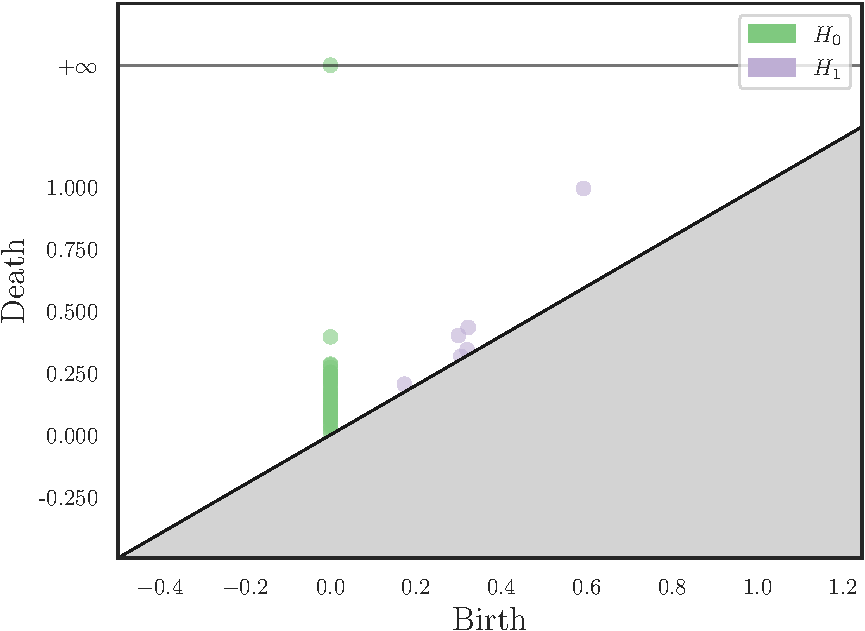
\includegraphics[scale=0.7]{diagram.pdf}
  \caption{\label{pdiagram} A persistence diagram over the birth and death of generators in the homology groups of a Vietoris-Rips complex approximated from points sampled from an annulus. The closer a point is to the diagonal line the shorter it lived. }
\end{figure}

  \section{Metrics}
  As persistent homology is often used as a topological summary of some data, it can be beneficial to be able to compare two different data samples with respect to their persistent homology. There are two commonly used metrics for doing this, the bottleneck distance and the Wasserstein distance.
  \begin{definition}
    The \textbf{bottleneck distance} between two persistence diagrams $X,Y$ is
    \[W_{\infty}(X,Y) = \inf_{\beta: X \to Y} \sup_{x \in X} ||x-\beta(x)||_{\infty}\]
    where $\beta$ is a bijection from $X$ to $Y$.
  \end{definition}
In other words, the bottleneck distance finds a matching, in the space of possible matchings, between the two persistence diagrams such that the largest distance in the matching is the smallest one possible. Since there could be more intervals in one persistence diagram, any point can also be matched with an infinite number of points on the diagonal which are included in the persistence diagram. Its name is derived from the fact that there is only one matching of points which contributes to the actual value of the distance, the largest one, and hence the distance is ``bottlenecked'' by that matching.

One disadvantage of the bottleneck distance is that it is quite coarse, it does not tell us very much about the other distances between other matched points. An alternative is the $q$-Wasserstein distance which instead incorporates all distances in the best matching.
  \begin{definition}
    The q-Wasserstein distance between two persistence diagrams $X,Y$ is
    \[W_{q}(X,Y) = (\inf_{\beta: X \to Y} \sum_{x \in X}  ||x-\beta(x)||_{\infty}^{q})^{\frac{1}{q}}\]
  \end{definition}
  Both the Wasserstein and bottleneck distance have their role as the bottleneck distance can be considered more robust to noise, since small changes in the matchings are ignored in favor of the largest matching.

  A desired quality of these metrics are stability, ideally we want the metrics to actually reflect difference in the underlying spaces. There are stability theorems that under varying conditions fulfill a meta-theorem which guarantee this.

  \begin{definition}
    A filtration function $X \to \mathbb{R}$ is a function from a simplicial or cubical complex $X$ such that the sublevel set $\{ f^{-1}(-\infty,a) \mid a \in \mathbb{R} \}$ is a filtration.
  \end{definition}

  \begin{theorem}[Stability meta-theorem \cite{vejdemo}]\label{stab}
    For a nice enough space $X$ and nice enough filtration functions $f,g: X \to \mathbb{R}$, a nice enough norm of the difference of $f-g$ serves as an upper bound to the distances between the persistence diagrams given by $f,g$.
  \end{theorem}

  In other words, a small perturbation of the filtering functions will at most be as large as the difference between the functions themselves. The term \textit{nice} is intentionally vague, since these conditions vary. For an overview of the particular scenarios in which the meta-theorem is applicable see \cite{vejdemo}, including a formulation which allows for general persistence modules under certain conditions. In our practical applications we are only considering finitely many sublevel sets from a filtration function which motivates the following definition.

  \begin{definition}
    A filtration is called \textbf{tame} if the persistence complex arising from the filtration function is of finite type.
  \end{definition}

Then we have the following corollary of the meta-theorem.

  \begin{corollary}\label{stabtame}
    If $f,g$ given as in Theorem \ref{stab} are \textit{tame} then the meta-theorem holds for the bottleneck distance with norm given by the $L_{\infty}$-norm and for the $q$-Wasserstein distance with the $L_{q}$-norm.
  \end{corollary}
  As the proofs of Corollary \ref{stabtame} require a lot of tedious and technical details which would detract from the overall theme of this thesis, we instead refer the reader to elementary proofs regarding the $q$-Wasserstein distance in \cite{skraba2021wasserstein} and the bottleneck distance in \cite{skraba2021notes}.
%%% Local Variables:
%%% mode: latex
%%% TeX-master: "thesis.tex"
%%% End:

\chapter{Two Applications of Persistent Homology}

Since our purpose with thesis is not only to give an introduction to persistent homology in terms of theory, but also display how it can be used with actual real-world data, we illustrate this pipeline two different case studies where persistent homology serve as our main tool for data analysis.

In the first case we quantify differences in morphology between different-sized individuals of the bumblebee \textit{Bombus terrestris} by computing the persistent homology of 3D volumes of their corneas. To our knowledge this is the first use of persistent homology in data pertaining to insects, although materials \cite{moon2019, delgadofriedrichs2014}, reconstructions of 3D volumes \cite{gutierrez2012, gutierrez2014} and plants \cite{plants} have been investigated with approaches that are similar in spirit.

In the second case we try to understand the network structure of the striatum, a part of the basal ganglia in the brain. Due to the sheer computational power needed to compute persistent homology for this data our analysis is more of a holistic summary of the resulting simplicial structure rather than focusing solely on persistent homology. Our approach is largely inspired by \cite{reimann}, in which a similar analysis is done but for a different part of the brain.

The application of persistent homology to a data-set is not entirely trivial. In order to compute persistent homology we need to construct a persistence complex on the data at hand. This can be done in a multitude of ways, but the basic pipeline can be seen in Figure \ref{pipeline}.

\begin{figure}[h]
  \centering
  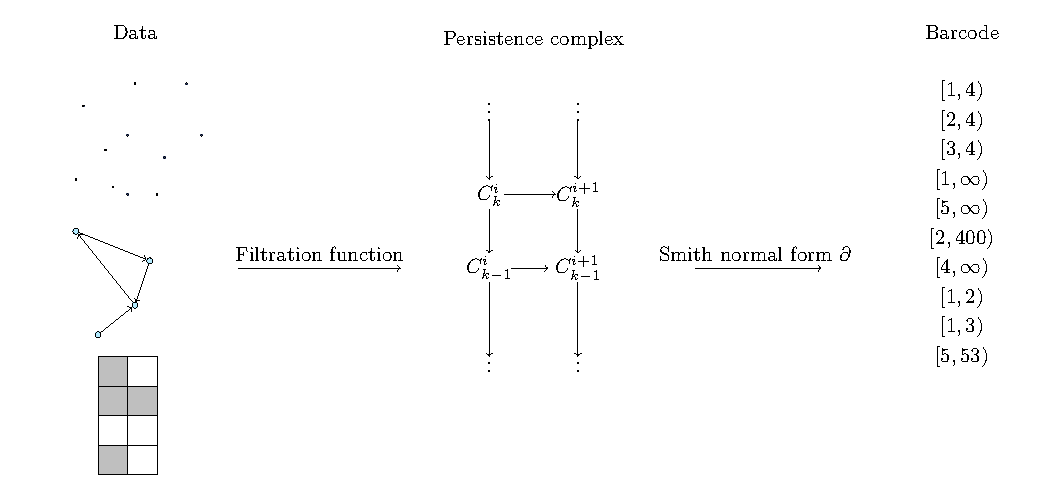
\includegraphics[scale=0.8]{pipeline.pdf}
  \caption{\label{pipeline} The pipeline of computing persistent homology of data.}
\end{figure}

A central part of this pipeline is the formulation of a filtration function which yields a sequence of complex and hence a persistence complex. The filtration provides the translation of data into an algebraic object we can compute persistent homology of. This means that when we analyze results from persistent homology, perhaps by comparing metrics between two barcodes or reading directly of a persistence diagram, the semantic meaning of those results is intimately connected to how the filtration creates the resulting complex. Dually, this means that in order to formulate the filtration we need to have a strong understanding of the data itself so that our filtration captures essential properties of the data. The complex constructed on the data-set is an approximation of it topologically, but since it is not the ``true'' space in which the data lives care has to be taken so that any conclusions made from the barcode are meaningful.


\section{Corneas of Bombus terrestris}
It has been found that the size of individuals of the species \textit{Bombus terrestris} affects aspects of their visual capabilities \cite{emily}. By applying persistent homology we can investigate whether this difference in size also translates to a difference in persistent homology, and so by proxy a difference in topology. If so, this could serve to strengthen the hypothesis that larger individuals have superior, or at the very least different, visual capabilities than smaller individuals. Persistent homology is a good candidate for this purpose as metrics on persistence diagrams are indifferent to differences in scale but rather measures differences in shape.

Our questions we wish to investigate in this case study are
\begin{enumerate}
  \item Is there a correlation between the size of the bumblebees and their persistent homology?
  \item Can we with persistent homology identify subgroups of bumblebees, and if so are these subgroups related to their size?

\end{enumerate}
\subsection{Data}
The data consists of binary 3-dimensional volumes (see Figure \ref{corneas} for renderings of some of the samples) of the corneas acquired by micro-CT scans of the samples described in Table \ref{bees}. The main focus of the analysis will be on samples from the bumblebee \textit{Bombus terrestris}, but in total there are 20 samples belonging to 8 different species of insects. The additional samples from other species will be used to verify our topological findings.
\begin{figure}[h]
  \centering
  \begin{subfigure}{.3 \linewidth}
  \centering
  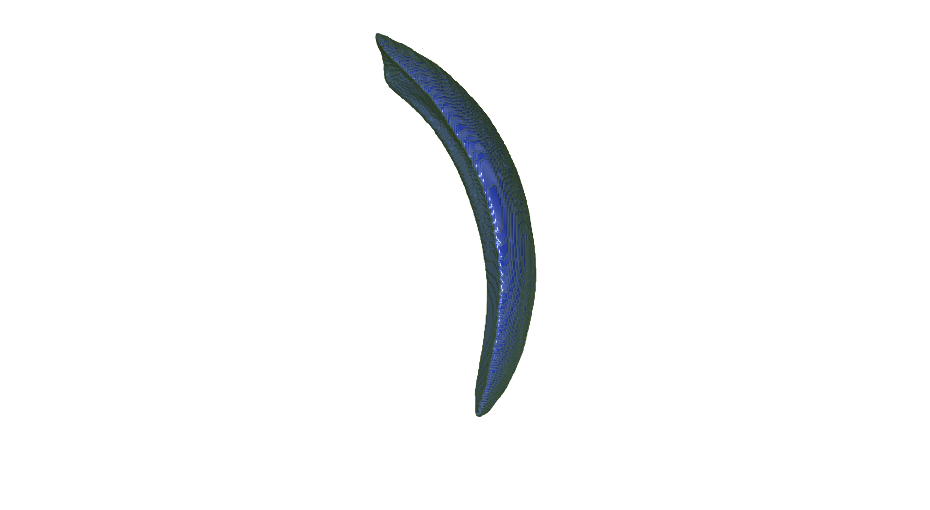
\includegraphics[scale=0.2]{ta60204_cornea.png}
  \caption{TA\_60204}
  \end{subfigure}%
  \begin{subfigure}{.3 \linewidth}
  \centering
  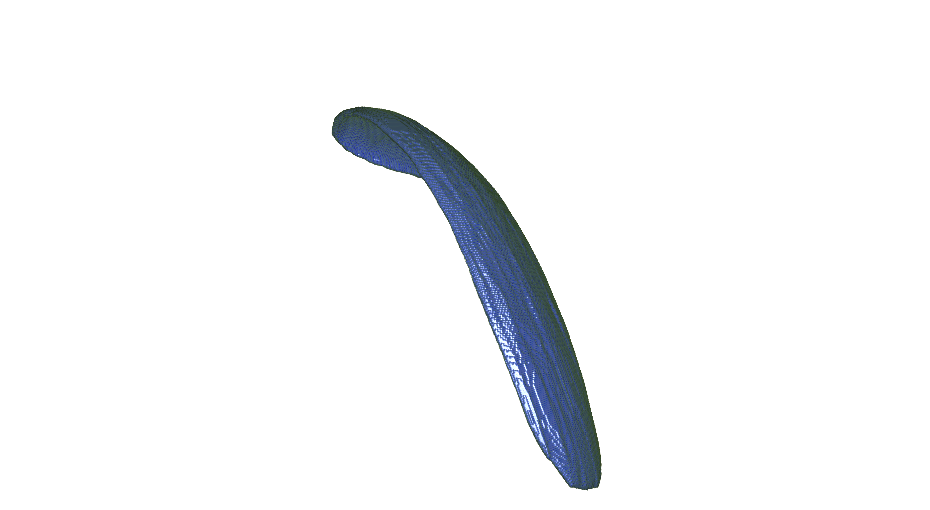
\includegraphics[scale=0.2]{mq60209_cornea.png}
  \caption{MQ\_60209}
  \end{subfigure}%
  \begin{subfigure}{.3 \linewidth}
  \centering
  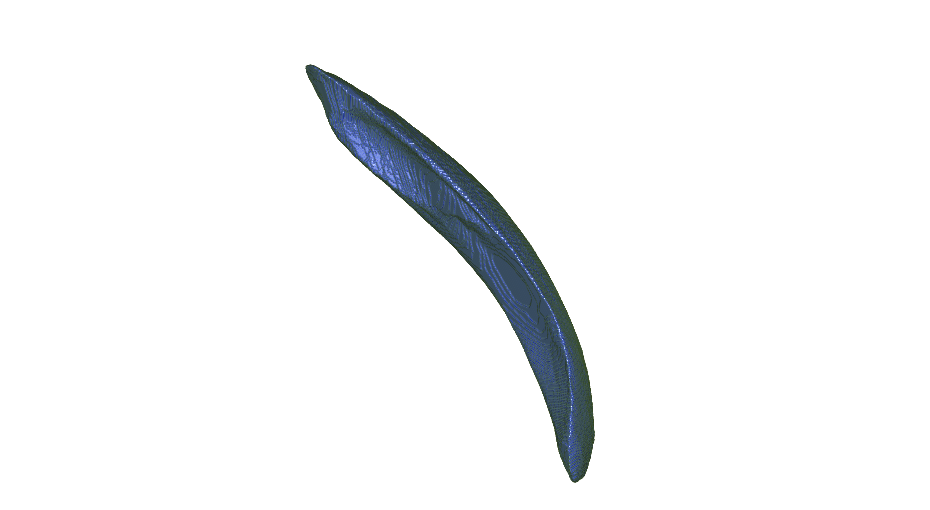
\includegraphics[scale=0.2]{bt77970_cornea.png}
  \caption{BT\_77970}
  \end{subfigure}
  \caption{\label{corneas} Example renderings of cornea volumes.}
\end{figure}
\begin{table}[h]
\begin{center}
\begin{tabular}{*6l}
\toprule
  ID & ITW & Species  \\ \midrule
AM\_60185 & 2.90 & Apis mellifera \\
AM\_60186 & 2.95 & Apis mellifera \\
BT\_77967 & 5.42 & Bombus terrestris \\
BT\_77970 & 4.00 & Bombus terrestris \\
BT\_77971 & 4.02 & Bombus terrestris \\
BT\_77973 & 1.97 & Bombus terrestris \\
BT\_77974 & 2.97 & Bombus terrestris \\
BT\_77976 & 5.47 & Bombus terrestris \\
MB\_60160 & 3.25 & Melipona bicolor \\
MB\_60161 & 3.25 & Melipona bicolor \\
MQ\_60208 & 3.64 & Melipona quadrifasciata \\
MQ\_60209 & 3.64 & Melipona quadrifasciate \\
PR\_60164 & 1.49 & Plebia remota \\
PR\_60206 & 1.49 & Plebia remota \\
TA\_60204 & 1.17 & Tetragonista angustula \\
TA\_78016 & 1.17 & Tetragonista angustula \\
TC\_60166 & 1.94 & Tetragona clavipes \\
TC\_60167 & 1.94 & Tetragona clavipes \\
TS\_60163 & 2.10 & Trigona spinipes \\
TS\_60203 & 2.10 & Trigona spinipes \\
  \bottomrule
\end{tabular}
\caption{Table over the data samples used in the analysis. The ID column gives a unique ID to each sample and the ITW column gives the intertegular width of each sample.}
\label{bees}
\end{center}
\end{table}
\subsection{Methodology}
Since the data we are working with are 3-dimensional volumes a natural choice is to endow it with the structure of a cubical complex. Our strategy is similar to the Vietoris-Rips complex, but instead of working with distances between points we work with adjacent cubes. Each voxel can be considered as a degenerate interval (or vertex) in a cubical complex, where $4$ pairwise adjacent voxels give rise to a square and $8$ pairwise adjacent voxels give rise to a cube.

In order to compute persistent homology we need a filtration which defines subcomplexes of the cubical complex. Since the volumes are binary, we give the volume a bit more structure by giving each voxel the distance to the closest point on the boundary of the volume.
\begin{definition}
  Given a subset $Y \subset \mathbb{R}^{n}$ we define the Euclidean Distance Transform, or EDT, as
   \[EDT(x) = \inf_{y \in \partial Y} ||x - y||_2\]
   where $\partial Y$ is the boundary of $Y$.
\end{definition}

Our filtration is a sequence of cubical complexes $K_{i}$ given by including voxels of at most value $\epsilon_{i}$ as degenerate intervals. Higher dimensional cubes such as edges, squares and geometric cubes are, similarly to the Vietorix-Rips complex, included whenever there is a sufficient amount of pairwise adjacent voxels.

\begin{example}
  To calculate the EDT of the binary image in Figure \ref{edt} we simply calculate the difference vector from a pixel of value $1$ to the closest pixel with value $0$. For example, to get $\sqrt 5$ in the top left corner we need to walk one step in to the left and two steps upwards which translates to the vector $(-1,2)$ which has Euclidean norm $\sqrt{1+4}=\sqrt{5}$. We then compute the filtration of the transformed image, which gives us cubical complexes for each value of $\epsilon$. Since there are five distinct values of the pixels, we find  five subsequent cubical complexes ordered by inclusion.

  \begin{figure}[ht]
    \centering
    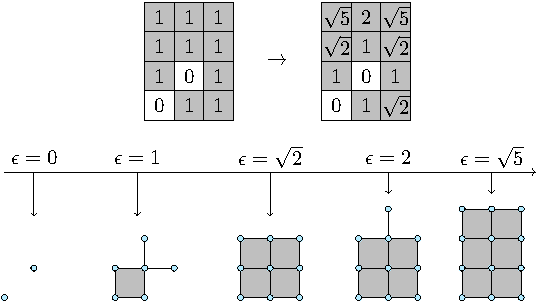
\includegraphics[scale=1]{cubicalfiltration.pdf}
    \caption{\label{edt} Transformation of a binary image into a filtration of cubical complexes based on the Euclidean Distance Transform.}
  \end{figure}

\end{example}

Our filtration on the volumes will describe the structure of the cornea starting at it the void surrounding it, then including the hollow shell which is its boundary, and then as the threshold increases the cubical complex will include more and more of the denser parts within the volume. An illustration of the thresholding at different values is seen in Figure \ref{thresh}.

\begin{figure}[ht]
  \centering
  \begin{subfigure}{.3 \linewidth}
  \centering
  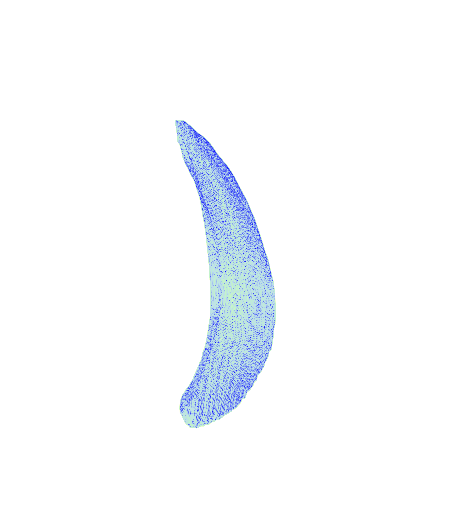
\includegraphics[scale=0.2]{eps2.png}
  \caption{$\epsilon < 2$}
  \end{subfigure}%
  \begin{subfigure}{.3 \linewidth}
  \centering
  
\includegraphics[scale=0.2]{eps10.png}
  \caption{$\epsilon < 10$}
  \end{subfigure}%
  \begin{subfigure}{.3 \linewidth}
  \centering
  
\includegraphics[scale=0.2]{eps100.png}
  \caption{$\epsilon < 100$}
  \end{subfigure}
  \caption{\label{thresh} EDT thresholding of BT\_77976. Cooler colors indicate denser parts of the volume relative to the rest of the volume.}
\end{figure}

The resulting topological summaries we get are persistence diagrams. While these are in themselves interesting, in order to answer whether there is any relation between the size of an individual and the persistent homology of its cornea, we compute a distance matrix giving the distance of each sample to another. Since we have a number of dimensions of homology to compare and two different metrics (1-Wasserstein and Bottleneck) we get a total of 6 distance matrices. For each of these distance matrices, we divide them into two submatrices, one group consisting of the submatrix with entries from \textit{Bombus terrestris} and the other group consisting of all the other samples to act as a control group on the first.

Our hypothesis is that there is some relationship between the distances given by the absolute difference in ITW and their persistent homologies. But since different homology dimensions and metrics provide different summaries of the objects we first need to figure out which one of them is most suited for our applications.

We determine which metric we will rely on by doing a so called \textbf{Mantel test} of the distance matrix with respect to homology and the distance matrix with respect to ITW. A Mantel test is a non-parametric test of distance matrices, in which we compute the Spearman rank correlation of the two matrices under the null hypothesis that the matrices are uncorrelated. We can then derive a test statistic by permuting one of the matrices in both rows and columns and computing correlations for each such permutation.  The results of a Mantel test is a correlation coefficient indicating the strength of the correlation and $p$-value indicating how likely it is  that this coefficient would appear in a random permutation of one of the matrices.

We then perform clustering of the persistent homology distance matrix based on \textbf{hierarchical clustering}. It is a simple algorithm where we first consider each sample as its own cluster, and then group together clusters depending on the distance between them. The distance between two clusters is given as the minimum distance between any two samples between the two clusters. Our hope then is that the final clustering, based on persistent homology, reflects the ITW of the \textit{Bombus terrestris} samples.


\subsection{Results}
The Mantel tests in Table \ref{mantelc} reveal that the highest correlation is given by the bottleneck distance on $H_{2}$. Perhaps this is not too surprising, our objects are volumes and the most distinguishing aspects of volumes will be how they encode voids. Interestingly, the $H_{1}$ bottleneck distance matrix shows a very high $p$-value indicating that the largest distance between holes is not very telling in drawing a conclusion about correlation between size and persistent homology. This could be explained again by the fact that our object is a volume of a single connected component namely a cornea, and so any existence of holes will at best be local geometric information and at worst simply noise.

\begin{table}[h]
\begin{center}

\begin{tabular}{*6l}    \toprule
Group  & Metric  & $H_{1} \rho $  & $H_{1}$ p-value  & $H_{2} \rho$ & $H_{2}$ p-value  \\ \midrule
\textit{BT} & Bottleneck & $-0.069$ & $0.84$ & $0.86$ & $0.0083$\\
\textit{BT} & Wasserstein & $0.59 $ & $0.053 $ & $0.49$ & $0.080$\\
\textit{Others}& Bottleneck & $0.22$ & $0.030$ & $0.33$ & $0.0073$\\
\textit{Others}& Wasserstein & $0.23$ & $0.023$ & $0.26$ & $0.013$\\\bottomrule
 \hline
\end{tabular}
\end{center}

\caption{\label{mantelc} Table displaying the statistics computed in the Mantel test of the pairwise distances in different dimensions of persistent homology and the ITW for the species \textit{Bombus terrestris}. The symbol $\rho$ denotes the Spearman rank correlation coefficient computed between the two distance matrices. }
\end{table}

The $1$-Wasserstein metric does not provide a low enough $p$-value for us to draw any conclusions from the tests when it comes to \textit{Bombus terrestris}, this perhaps indicates that the sample size of the \textit{Bombus terrestris} submatrix is too small. It is possible that the more sensitive nature in the $1$-Wasserstein metric, since it records not only the largest differences in the persistence diagrams but all of them, makes it less robust to a smaller sample size.

Since the bottleneck distance on $H_{2}$ has a strong correlation with the ITW distance matrix we proceed with a hierarchical clustering on its distance matrix as seen in Figure \ref{h2b}. We see that there are two groups formed where one of the groups contains an additional cluster. The first group, which does not contain a subgroup, consists of two samples BT\_77967 and BT\_77976. These are the largest samples in terms of ITW and the remaining group contains two subgroups both in which the ITWs are smaller. It is worth repeating that this clustering is done without knowledge of the actual ITW, these clusterings are purely based on the bottleneck distance of the $H_{2}$ persistent homology and as such a differences here indicate differences based solely on the fact that their persistence diagrams differ.

\begin{figure}[ht]
  \centering
  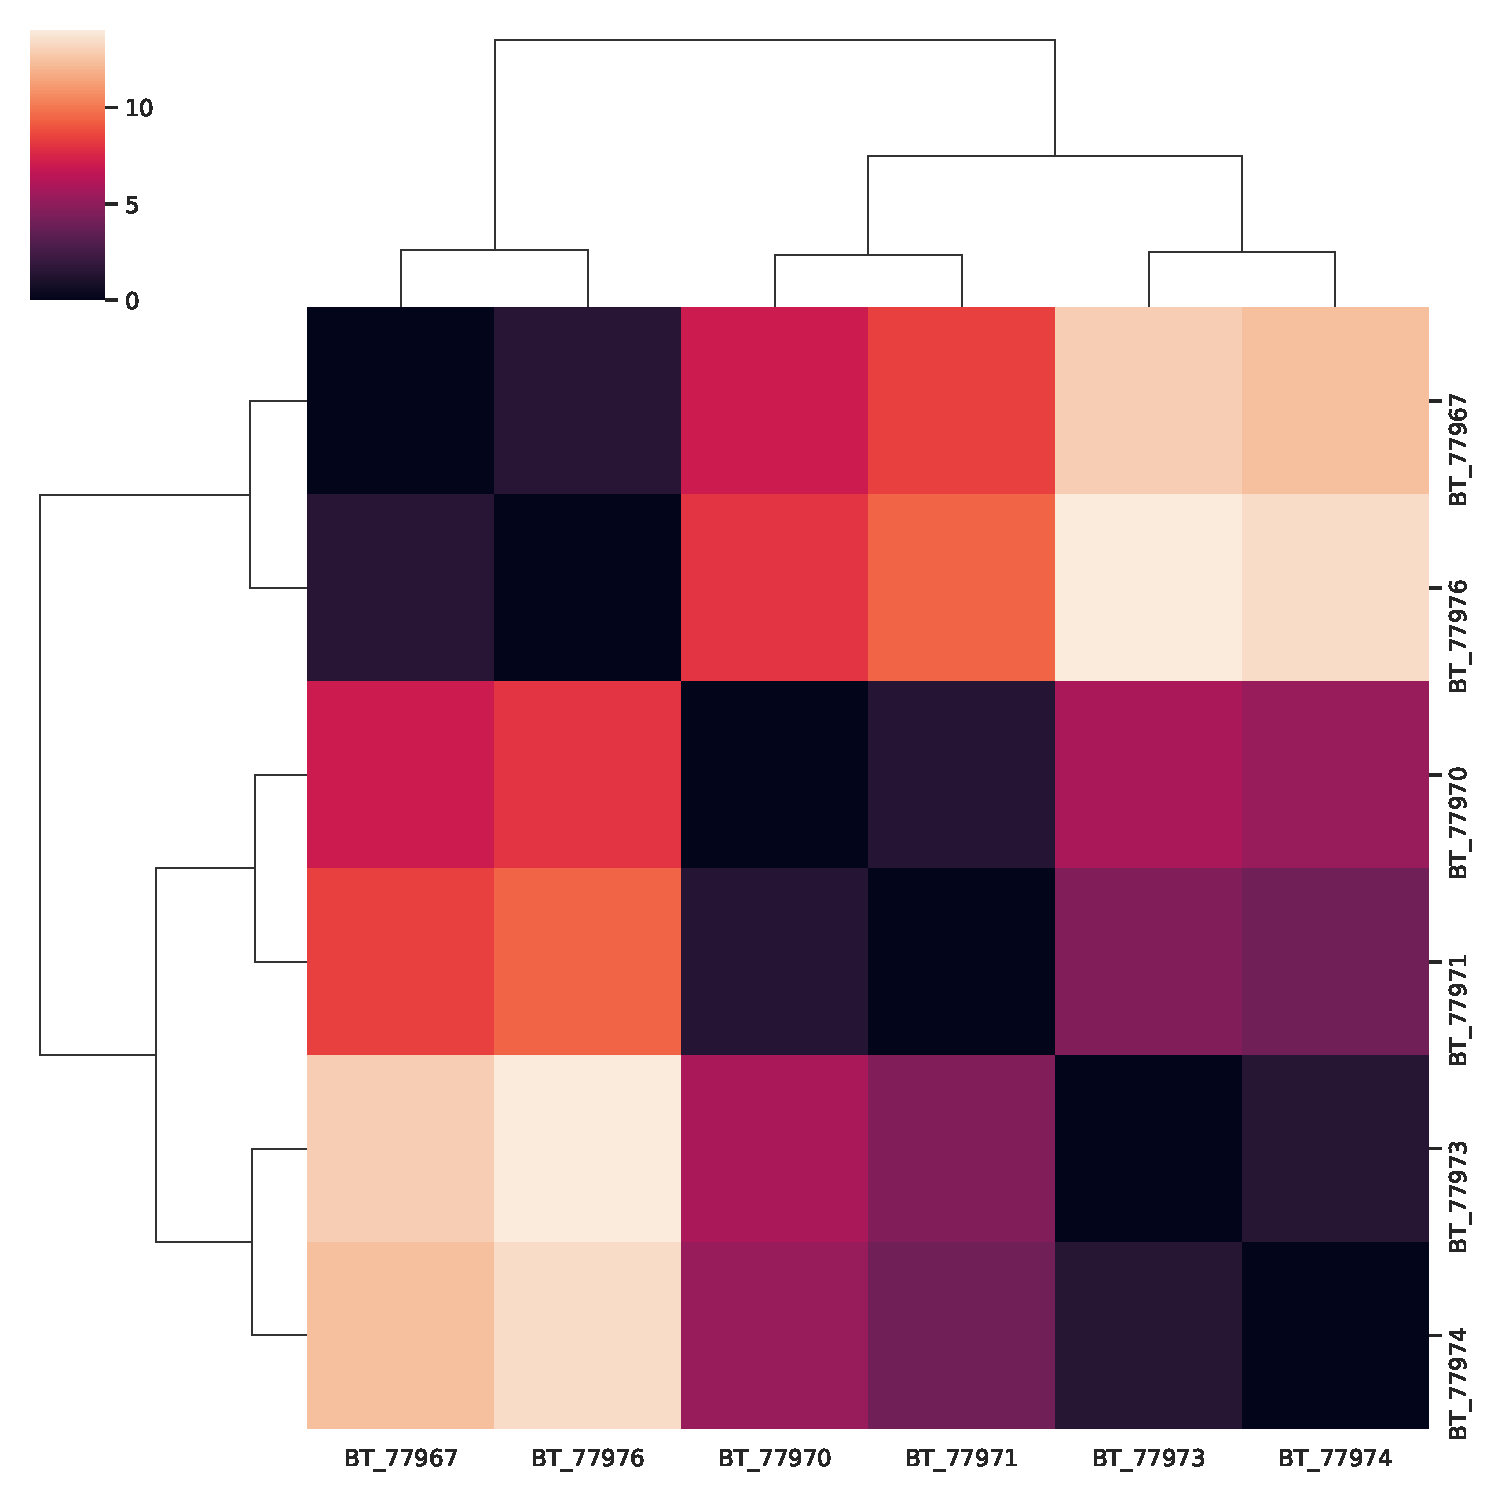
\includegraphics[scale=0.35]{clusters/bottleneck_h2_cluster.pdf}
  \caption{\label{h2b} Hierarchical single-link clustering of the bottleneck distance matrix derived from the persistent homologies of the \textit{Bombus terrestris} in $H_{2}$.}
\end{figure}

In order to further clarify in what way the persistence diagrams of the \textit{Bombus terrestris} are differing we can look at visualizations of the bijections done under the bottleneck distance and which pair of generators are the ones to determine the metric.

In Figure \ref{ingroup-matching} we see the matchings produced for the elements \textit{within} each of the identified clusters. We see that within the group the optimal matching always gives the largest distance as a matching between a point and the diagonal.

On the other hand, if we look at the distances from samples \textit{between} groups in Figure \ref{outgroup-matching} we see that there is one generator that is responsible for the bottleneck distance in all of these matchings. That is the longest living generator which is born at filtration value $0$. At filtration value $0$ the only voxels in the volume are the empty voxels constituting the background, which means that the void is left by the space where the cornea will be at a higher filtration value. As the filtration value increases the volume gets filled in with denser and denser parts of the cornea, but as seen in Figures \ref{ingroup-matching} and \ref{outgroup-matching} it lives for a long time before the cornea is entirely filled out. This difference in lifetime, which can somewhat be translated to the density of the cornea, appears to be the distinguishing factor between the three identified clusters of samples.

\begin{figure}[ht]
  \centering
  \begin{subfigure}{.49 \linewidth}
  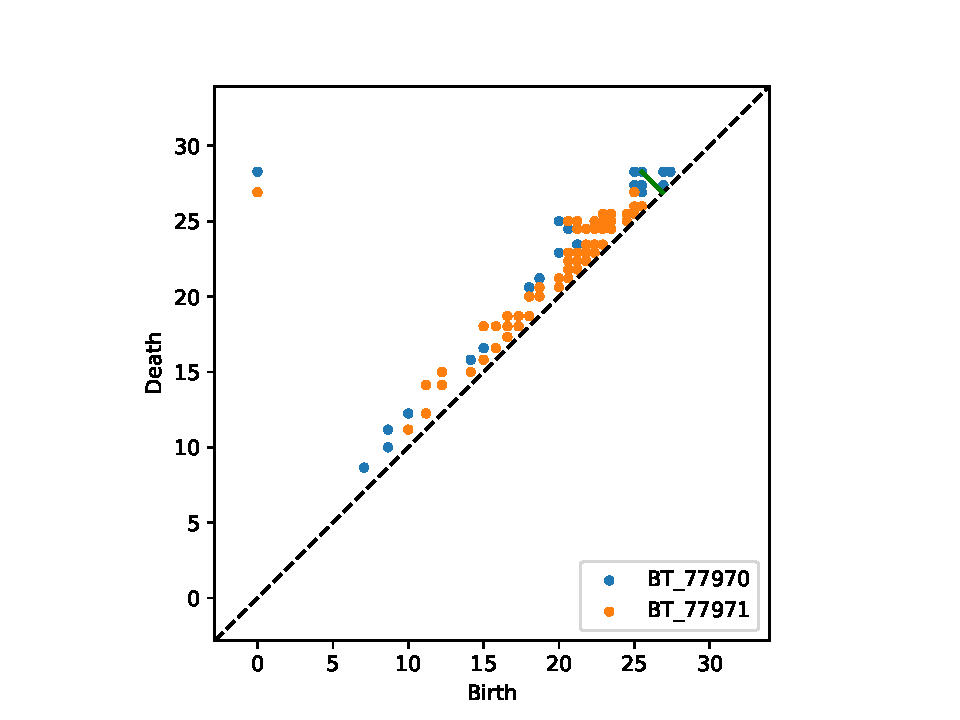
\includegraphics[scale=0.5]{matchings/77970-77971.pdf}
  \end{subfigure}%
  \begin{subfigure}{.49 \linewidth}
  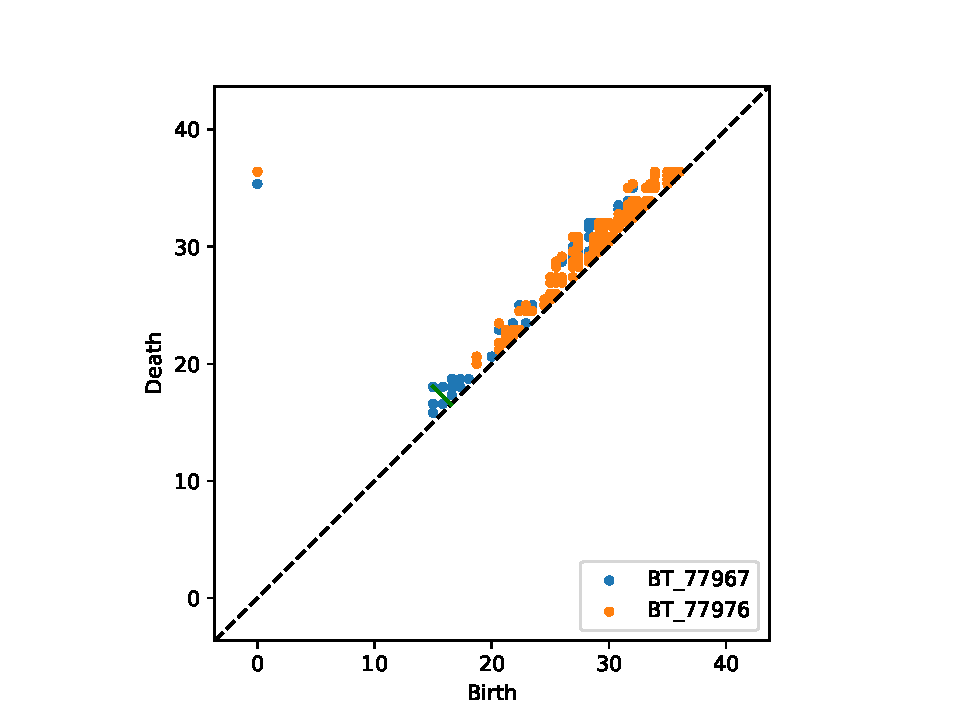
\includegraphics[scale=0.5]{matchings/77967-77976.pdf}
  \end{subfigure}
  \begin{subfigure}{.49 \linewidth}
  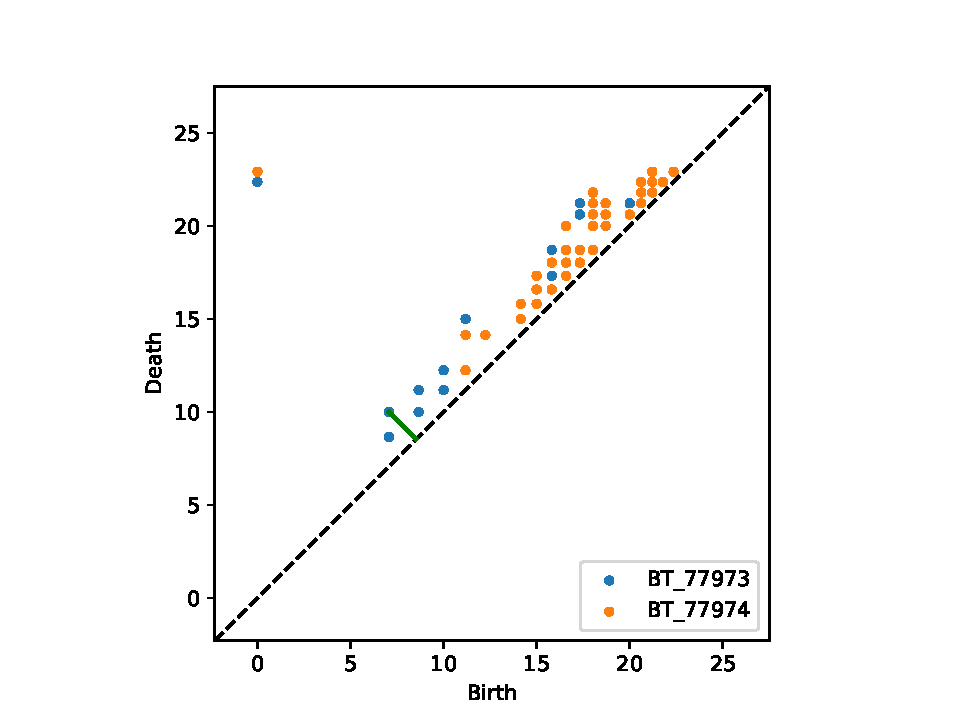
\includegraphics[scale=0.5]{matchings/77973-77974.pdf}
  \end{subfigure}
  \caption{\label{ingroup-matching} Visualisations of bottleneck distances within clusters on persistence diagrams of $H_{2}$.}
\end{figure}
\clearpage
\begin{figure}[ht]
  \centering
  \begin{subfigure}{.49 \linewidth}
  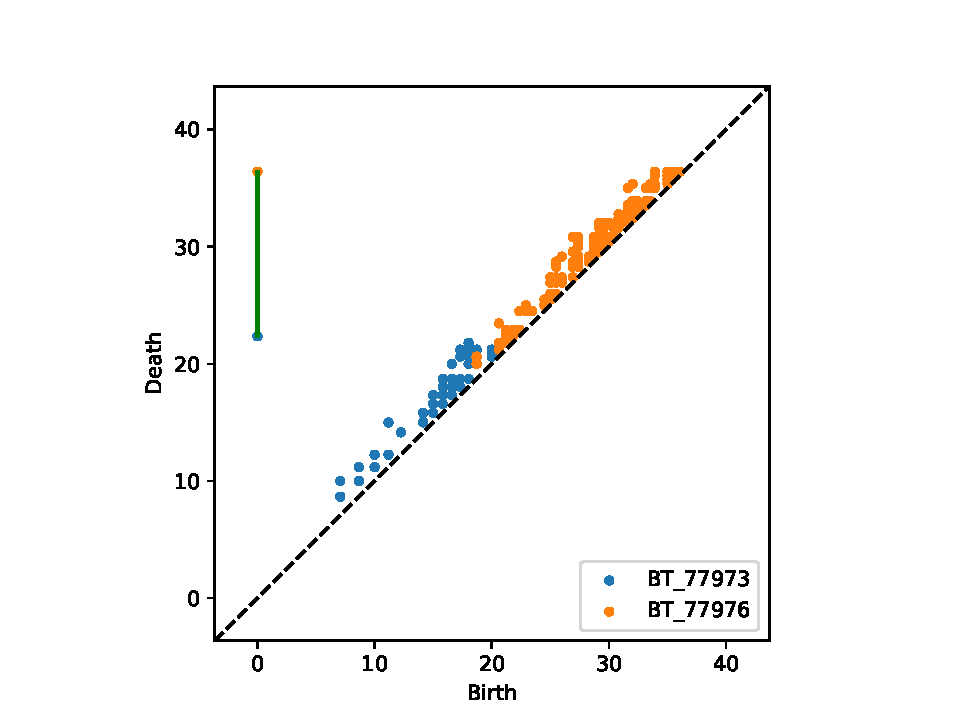
\includegraphics[scale=0.5]{matchings/77973-77976.pdf}
  \end{subfigure}%
  \begin{subfigure}{.49 \linewidth}
  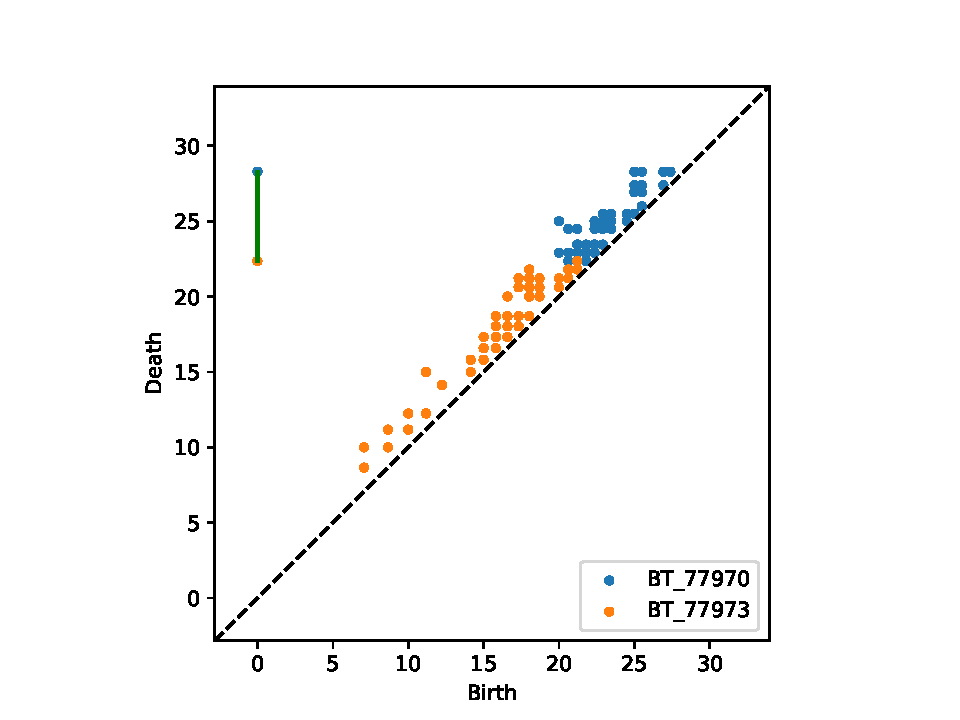
\includegraphics[scale=0.5]{matchings/77970-77973.pdf}
  \end{subfigure}
  \begin{subfigure}{.49 \linewidth}
  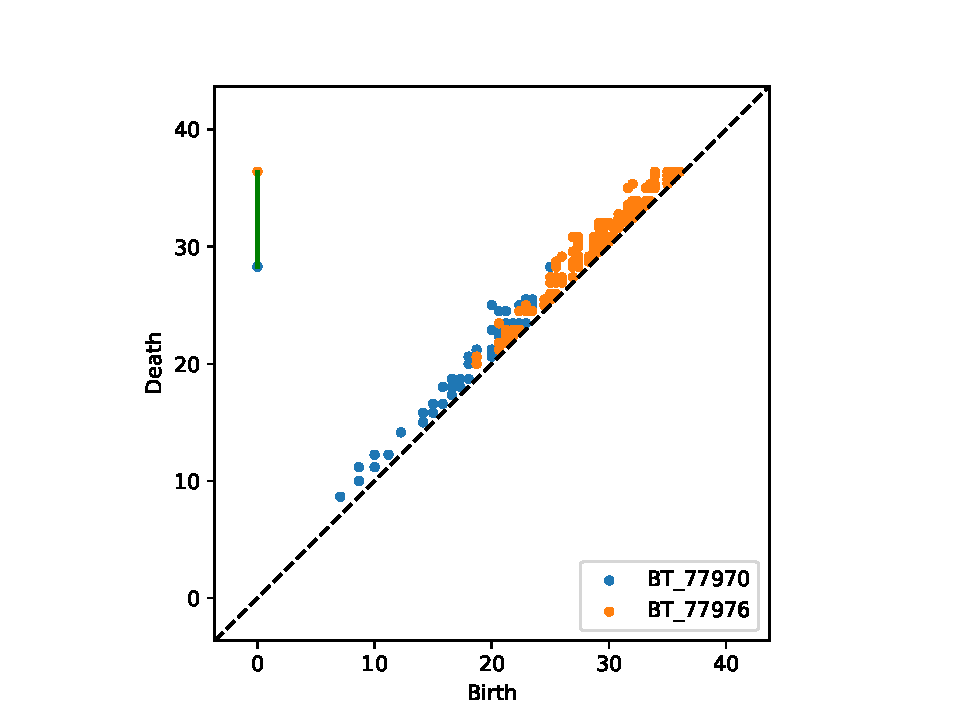
\includegraphics[scale=0.5]{matchings/77970-77976.pdf}
  \end{subfigure}
  \caption{\label{outgroup-matching} Visualisations of bottleneck distances between clusters on persistence diagrams of $H_{2}$.}
\end{figure}




While the purpose of this analysis is mostly to showcase persistent homology in the wild, these results  do support to the idea that different sized \textit{Bombus terrestris} do not only have larger eyes, but also that they are topologically different. Our clustering results on $H_{2}$ group the larger individuals together and we find a strong correlation with bottleneck distance in $H_{2}$ and ITW. Furthermore, we find that there is one generator born at the beginning of the filtration that is responsible for the ``bottleneck'' when comparing samples from the different clusters whereas within the same cluster other generators with much shorter lifetime are the contributors.
\clearpage
\section{The Simplicial Structure of the Striatum}
% The use of topological methods in order to understand brain networks is not new. There are a multitude of applications where persistent homology is used to overcome the problem of producing a graph from a set of a set sequence of connectivity maps by encoding all of them as a filtration. Traditional edge and vertex statistics have been generalized to simplices. Some other examples here.

There is much reason for considering simplicial complexes when it comes to networks related to the brain. An extensive field of study when it comes to network analysis of the brain are motifs, which at a high-level simply means a repeated pattern in a network which might have some form of semantic meaning to the network. Simplices capture such patterns at a micro-level through the connectivity of its faces. Furthermore, homology captures another type of patterns at a meso-level through cycles of simplices. Armed with persistent homology we arrive at a comprehensive summary of the network through the lens of the filtration of our choice.

In this analysis we follow \cite{reimann} by observing the high-dimensional simplicial structure of the brain by constructing a particular simplicial complex on the connectivity matrix of a synthetically generated microcircuit of the striatum as described in \cite{Hjorth202000671}, a part of the basal ganglia in the brain. By computing the resulting persistent homology we hope to discover distinguishing features of our network from a few selected control models. Furthermore, our aim is that this analysis serves as yet another example of the breadth of possible scenarios in which persistent homology is applicable outside the realm of theory. While we only investigate the mentioned microcircuit, our methodology is general enough for it to be applicable in any scenario where we data can be interpreted as directed graphs.

\subsection{Data}

Recall that a directed graph $G=\{V,E\}$ consists of a set of \textbf{vertices} $V$ and a set of \textbf{edges} $E$, where an edge is an ordered set $(v_{i},v_{j})$ for some vertices $v_{i},v_{j} \in V$. The \textbf{degree} of a vertex in a directed graph is the sum of the number of outgoing and incoming edges from and to the vertex.


In this case analysis our main object of study is a synthetic network of generated based on empirical findings regarding the micro-circuitry of the striatum realized as a directed graph, see \cite{Hjorth202000671} for further details. We compare this network to a three different models of directed graphs that all have different qualities common to networks of the brain.

\begin{definition}[{\cite{erdos}}]
The \textbf{Erdős–Rényi (ER) model} generates a directed graph through the choice of two parameters: the number of vertices $n$ and the number of edges $m$. The graph is then selected uniformly from the set of all graphs with $n$ vertices and $m$ edges.
\end{definition}

\begin{definition}[{\cite{strogatz}}]
The \textbf{Watts-Strogatz (WS)} model is parameterized by the number of vertices $n$, the average out-degree $m$ and a rewiring probability $p$. A directed graph is constructed by first creating a graph of $n$ vertices, such that for every vertex there is an outgoing edge to its $m$ closest neighbours modulo $n$, meaning that the graph is circular. Then finally each edge has a probability $p$ of being rewired to a different, uniformly selected, endpoint.
\end{definition}

\begin{definition}[{\cite{barabasi}}]
  The \textbf{Barabási–Albert (BA) model} is parameterized by the number of vertices $n$ and $m$, the average out-degree of each vertex. It is constructed by first adding $m$ vertices and successively adding vertices until there are $n$ vertices. For each new vertex $v_{i}$ we add an edge $\{v_{i},v_{j}\}$  with a probability of
  \[
    \frac{\deg(v_{j})}{\sum_{k} \deg(v_{k})}
  \]
  Hence, at each addition of a vertex an older vertex with a high degree has a higher chance of having its degree increased.
\end{definition}
ER can be considered the baseline model, since it is an arbitrary random graph among all possible graphs. WS is said to have \textbf{small-world properties}, which means that there are clusters of highly connected nodes and that the average path between two vertices is short. BA is said to be \textbf{scale-free} which means that most vertices have a low degree, but some ``hubs'' have a high degree. Both scale-free and small-world properties have been observed in brain networks \cite{SPORNS2004418}. Figure \ref{graphexamples} gives an example of each model generated with $100$ vertices.

In this analysis we compare we will compare the three models above with the synthetic network generated from the striatum, which we will refer to as ST. In Table \ref{graphmodels} we can see our choice parameters for the models and the resulting number of edges and vertices. For ER and WS our parameter choices were made to match the number of edges in ST. However, for the BA model we instead choose parameters in order to match the number of dimensions in the simplicial complex on ST as seen in Figure \ref{count50k}.
\begin{figure}[ht]
  \centering
  \begin{subfigure}{.33 \linewidth}
    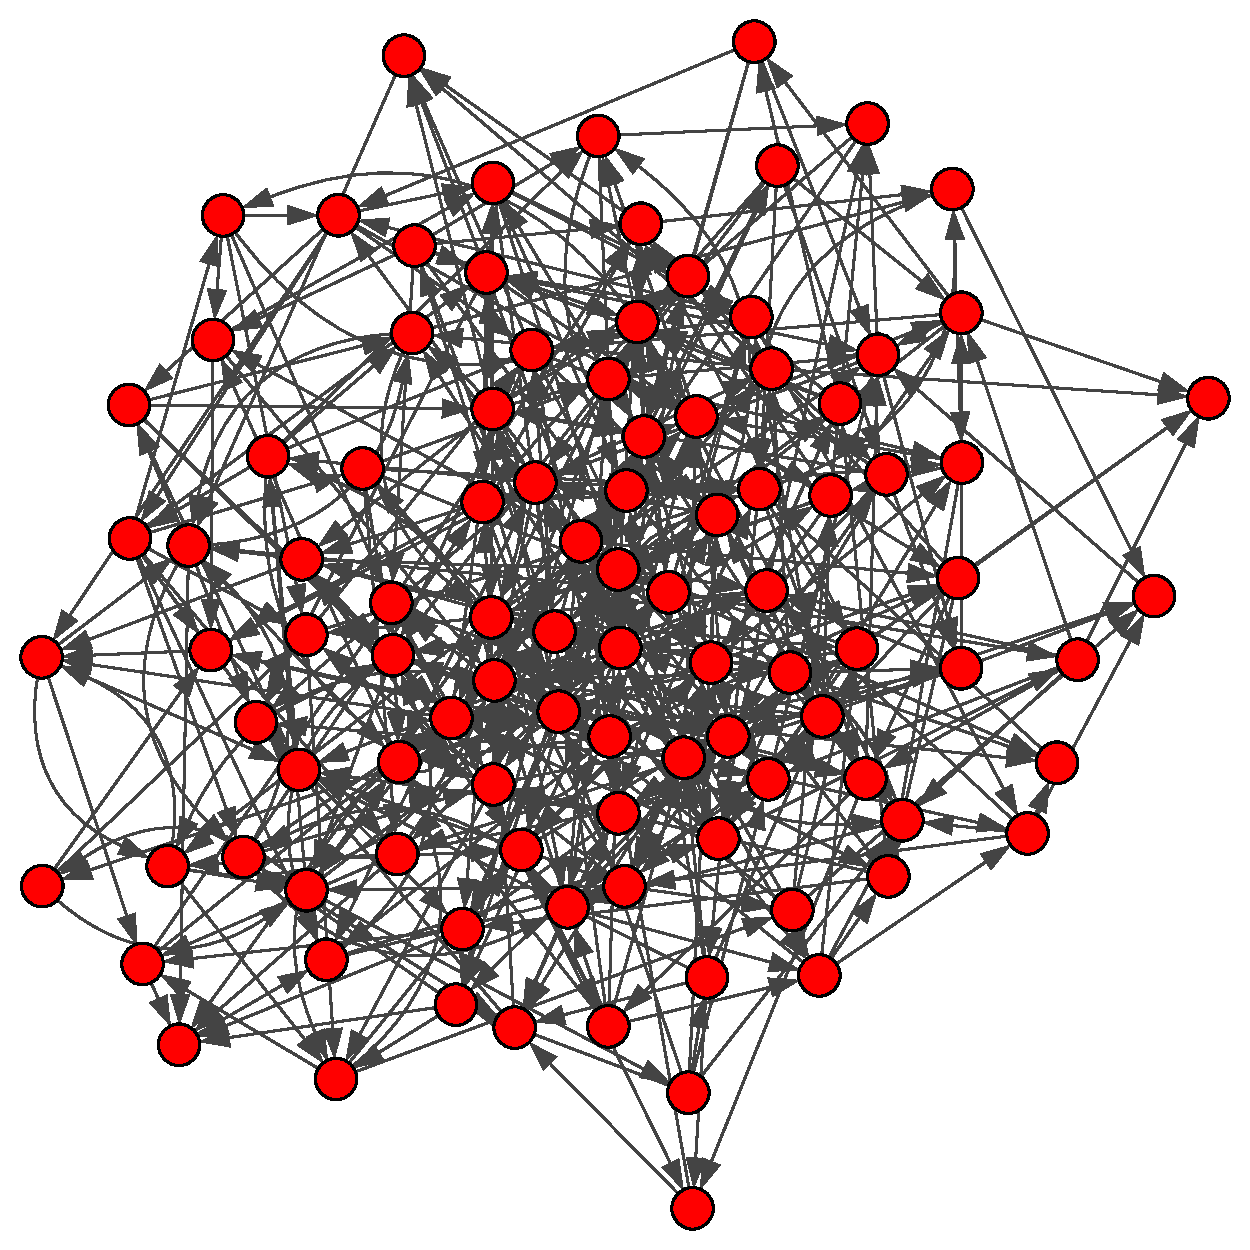
\includegraphics[scale=0.2]{random_graphs/erdos100v500e.pdf}
    \caption{Erdos-Rényi}
  \end{subfigure}%
  \begin{subfigure}{.33 \linewidth}

    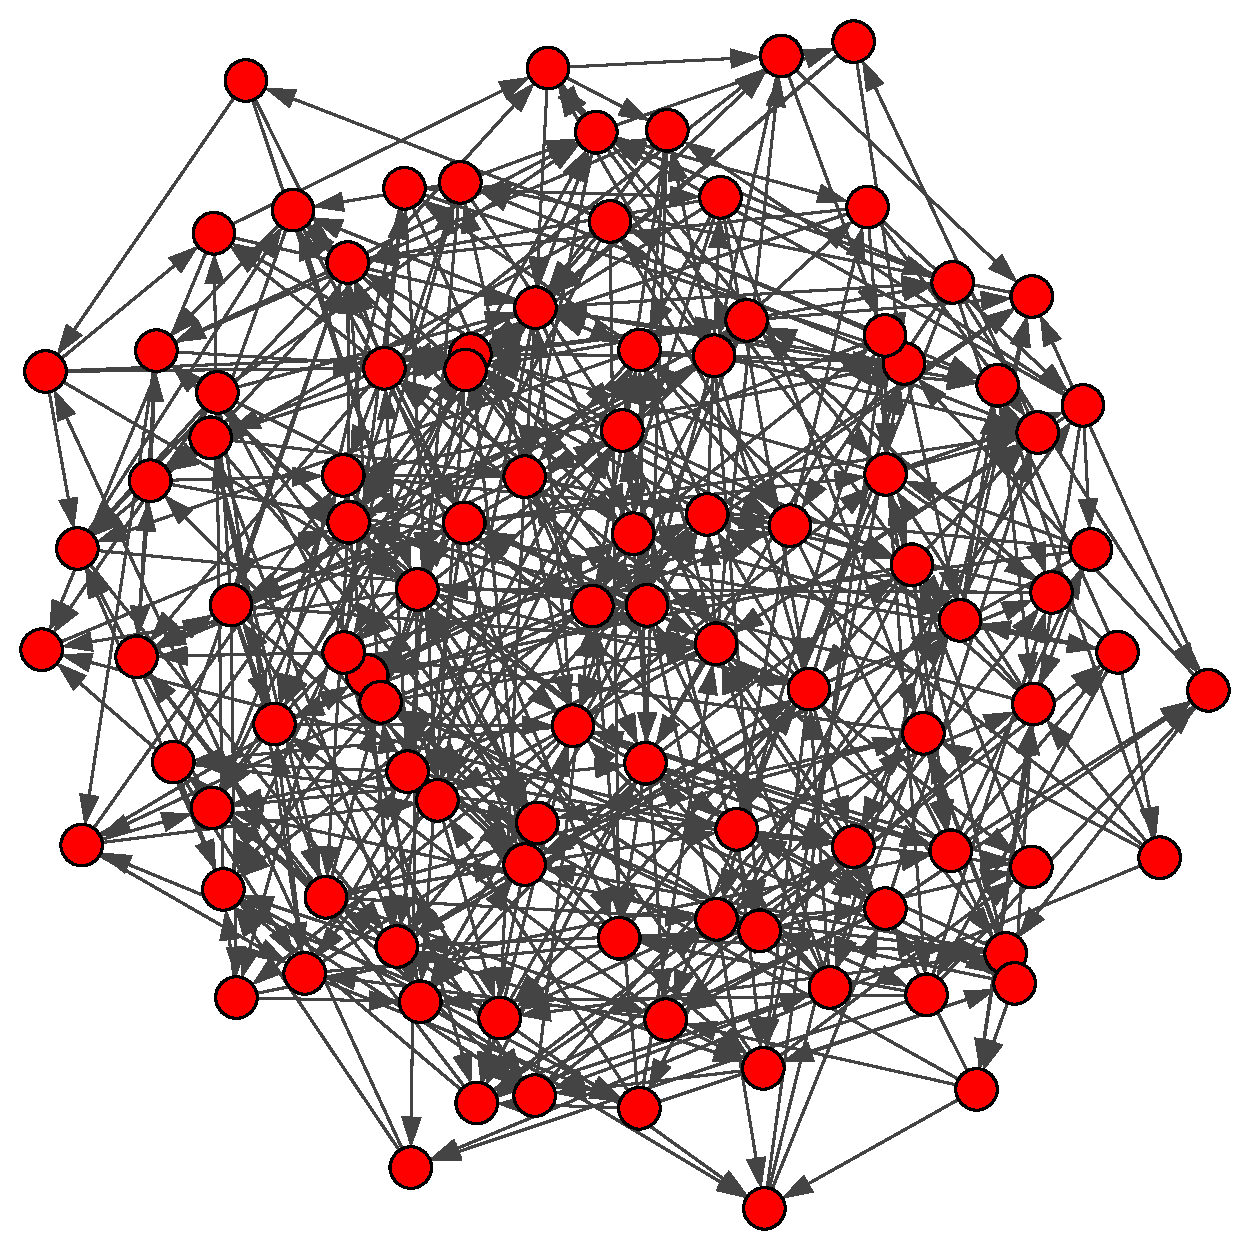
\includegraphics[scale=0.2]{random_graphs/strogatz100v5m05prob.pdf}
    \caption{Watts-Strogatz}
  \end{subfigure}%
  \begin{subfigure}{.33 \linewidth}

    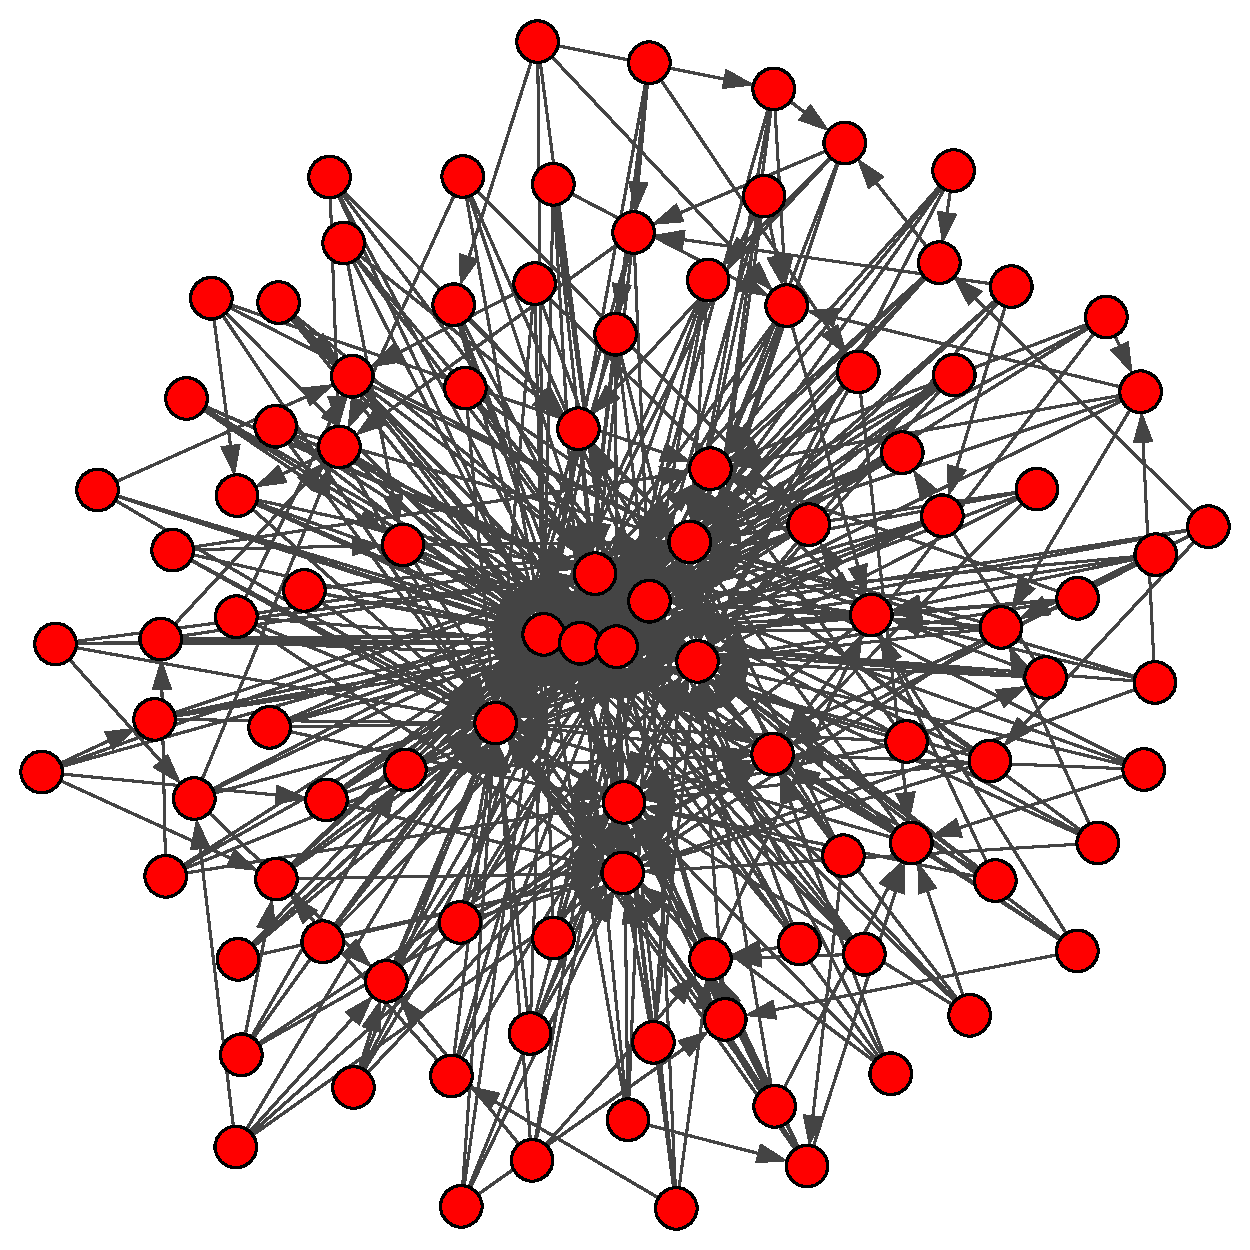
\includegraphics[scale=0.2]{random_graphs/barabasi100em5.pdf}
    \caption{Barabási-Albert}
  \end{subfigure}
  \caption{\label{graphexamples} An example of the ER, WS and BA models on 100 vertices.}
\end{figure}

\begin{table}[ht]
\centering
\begin{tabular}{*4l}    \toprule
  Network & Vertices & Edges & Parameters\\ \toprule
  ST & $50000$ & $12298074$  & - \\
  ER & $50000$ & $12298074$  & $n=50000, m=12298074$ \\
  WS & $50000$ & $12300000$  & $n=50000, m=247, p=0.5$  \\
  BA & $50000$ & $849864$ & $n=500000, m=17$
  \midrule
  \cr
  \bottomrule
\end{tabular}
\caption{\label{graphmodels} Breakdown of the ST, ER, WS and BA graphs compared in the analysis.}
\end{table}

\subsection{Methodology}
It is not entirely clear how we should define a simplicial complex on a \textit{directed} graph. The asymmetry is important as connections between neurons in the brain do not necessarily go both ways. While we could simply consider the network as a undirected graph by adding missing edges it is likely that important qualities of the network might be lost. There are a number of different ways to go about defining a similar complex on a directed graph . In our case we follow \cite{reimann} and construct something called the \textbf{directed flag complex} of a directed graph.

\begin{definition}[\cite{luetdigraph}]
  A \textbf{directed clique} is a directed graph $G=(V,E)$ such that every vertex has at least an outgoing or incoming edge to every other vertex in the graph. \end{definition}

Recall that an abstract simplicial complex as in Definition \ref{defabstractsimcomp} is given by ordered sets such that each subset of is also part of the entire complex. Hence, by taking a directed graph and introducing a partial order on the vertices we can construct an an abstract simplicial complex.

\begin{definition}[\cite{luetdigraph}]
  Let G=\{V,E\} be a directed graph. The \textbf{directed flag complex} dFl(G) is defined to be the simplicial complex whose $k$-simplices are all directed cliques with vertices $v_{0},\dots,v_{k}$ such that $\forall i: v_{i} \in V$
  and $\forall i,j: i < j \implies (v_{i}, v_{j}) \in E$. The vertices $v_{0}, v_{k}$ are called the source and the sink of a $k$-simplex.
\end{definition}

% Note that the directed flag complex adds two simplices for a bidirectional edge. This leads to the fact that we can have cycles given by the same vertex in the opposite direction. Normally, this is not the case.. since $[v_{0},v_{1}] = -[v_{1},v_{0}]$ in the ordinary simplicial complex whereas in the directed flag complex this is not true.

This construction is essentially the same construction given by the Vietoris-Rips complex where pairwise intersection is given by an edge. However, there are some notable difference due to the fact that the underlying graph is directed. One difference is that we only create a simplex from cliques of simplices whose edges flow ``upwards'' in the order. In Figure \ref{disimplex} we see how the left clique has a source and sink and thus defines a $3$-simplex in the directed flag complex, but the right clique has one edge going in the wrong direction hence it is not a $3$-simplex.

Another difference given by the fact that we have directions in the underlying graph, which for example results in that the simplices $[v_{0},v_{1}]$ and $[v_{1},v_{0}]}$ given by a bidirectional edge in the graph are two different simplices and hence make up a cycle $[v_{0},v_{1}]+[v_{1},v_{0}]$.
% It is important to try to understand this construction because it will have meaning when we try to interpret the homology of the resulting networks. In Figure \ref{disimplex} we see what a $3$-simplex looks like in a \textit{directed flag complex}. We then need to think about what a chain of these directed simplices look like. For example, a $2$-chain of directed simplices can be see in Figure \ref{}. Then what is a cycle? It is a cavity built in by these directed simplices. In the $1$-dimensional case it is not very difficult, it will look something like this.

\begin{figure}[ht]
  \centering
  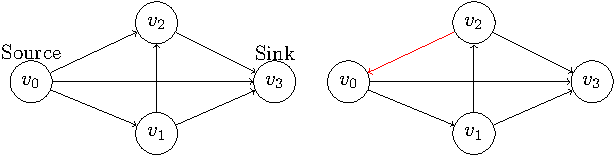
\includegraphics[]{./3simplex.pdf}
  \caption{\label{disimplex} Two directed cliques where the left clique does create a 3-simplex in the directed flag complex and the right clique does not.}
\end{figure}

We investigate the graphs ST, ER, WS, and BA in three different ways: the number of simplices in each dimension, their Betti numbers and their persistence diagrams.

For computing persistent homology, we need to define a filtration on the directed flag complexes.
We use a simple filtration function
\[
  f(\sigma) = \begin{cases}
    -\deg(\sigma) & \text{if } \dim(\sigma) = 0 \\
    \max_{\tau \text{ is a face of } \sigma} \{ f(\tau) \} & \text{if } \dim(\sigma) > 0
  \end{cases}
\] where we add vertices in the reverse order of their degrees and their resulting higher-dimensional simplices whenever all their vertices have been included in the complex. The degree of the vertex indicates how central a vertex is to the graph, which means that the filtration will describe the network in its most basic building blocks and then add less and less important vertices.
\subsection{Results}
First we note the large number of simplices in ST as seen in Figure \ref{count50k}, where we find as much as over a hundred billion simplices in dimension $7,8$ and $9$. This phenomena was also observed in \cite{reimann}, however not of the same magnitude.  Furthermore, we see that the number of dimensions is significantly larger in ST compared to ER and WS. The graph BA was chosen so that its directed flag complex had the same dimension as ST's, but we see that the number of simplices in each dimension is notably lower. So while the BA model seems to capture the complexity of connectivity in ST it does not capture the magnitude. ER and WS present a lot fewer simplices and a lot fewer dimensions than ST. In this sense ER is the simplest model, but this is to be expected since it is a random graph we expect there to be less of simplicial complexity.

One thing that has to be mentioned is that the computation of homology and even more so persistent homology becomes extremely computationally expensive due to the number of simplices in ST. As seen in Section 3.3 reducing the boundary matrix in a dimension is at worst case given by a cubical amount of field operations in proportion to the number of simplices in one dimension above. Hence, computing something like $\beta_{7}$ for ST would involve a computation of the magnitude $10^{3 \cdot 11}$ field operations. Even worse, in practice computation persistent homology is not only affected by the number of simplices in the resulting simplicial complex, but also the number of simplicial complexes in the filtration. For this reason we only present persistence diagrams and Betti numbers for $H_{0},H_{1}$ and additionally the Betti number for $H_{2}$.

In Table \ref{bettis} we see that ST has a lower $\beta_{1}$ than any of the other graphs. Curiously, even though BA has a lot fewer edges it still has a higher Betti number in dimension 1. It is possible that the low amount of $1$-cycles is a feature that distinguishes brain networks from other types of networks, but no such result is presented in \cite{reimann} since $\beta_{1}$ was never computed due to computational limitations. If we turn to $\beta_{2}$ we see that $ST$ has the largest change from $\beta_{1}$, while the other graphs are pretty close to their $\beta_{1}$ however with a larger error. This dramatic increase from dimension 1 to dimension 2, both in Betti number and number of simplices, could also be seen as a feature of $ST$ compared to the other models. The distribution of simplices in Figure \ref{count50k} hints that this dramatic increase likely continues for several dimensions.

We see in Figure \ref{graphph} that ST is markedly different from all other models in terms of persistent homology. The persistence diagram of $BA$ is not very informative due to all of its vertices essentially having the same degree. However, WS and ER display similar persistence diagrams in which the distribution of holes is concentrated to a small interval of filtration steps from degree $500$ to degree $400$. In comparison, ST shows a much larger spread of both birth and death of holes, with some holes even being born or dying close to degree $0$.

To conclude, we have found that directed flag complex on $ST$ differs in several ways from the other three graphs: it has a much larger number of simplices in each dimension, it has simplices in high dimensions, it has lower $\beta_{1}$ than all models and lower $\beta_{2}$ than all models but BA. Furthermore, the persistence diagram of ST shows a distinct spread of the birth and death of generators of $H_{1}$, whereas for BA they are all born at the same time due to nature of the filtration and for ER and WS they are all restricted within a small interval of degrees.
%To interpret this, we have to remind ourselves of the definition of a $1$-dimensional hole in the context of a directed flag complex. It will be a cycle of edges such that there is no $2$-simplex, which is a triangle with a source and sink, including it. For example, a hole could look like this or like this both being valid holes, however it cannot look like this. This means that when a hole is killed, a vertex was added that gave rise to a vertex which turned the hole into a cycle. This only happens when
\begin{figure}[ht]
  \centering
  \begin{subfigure}{.49 \linewidth}
    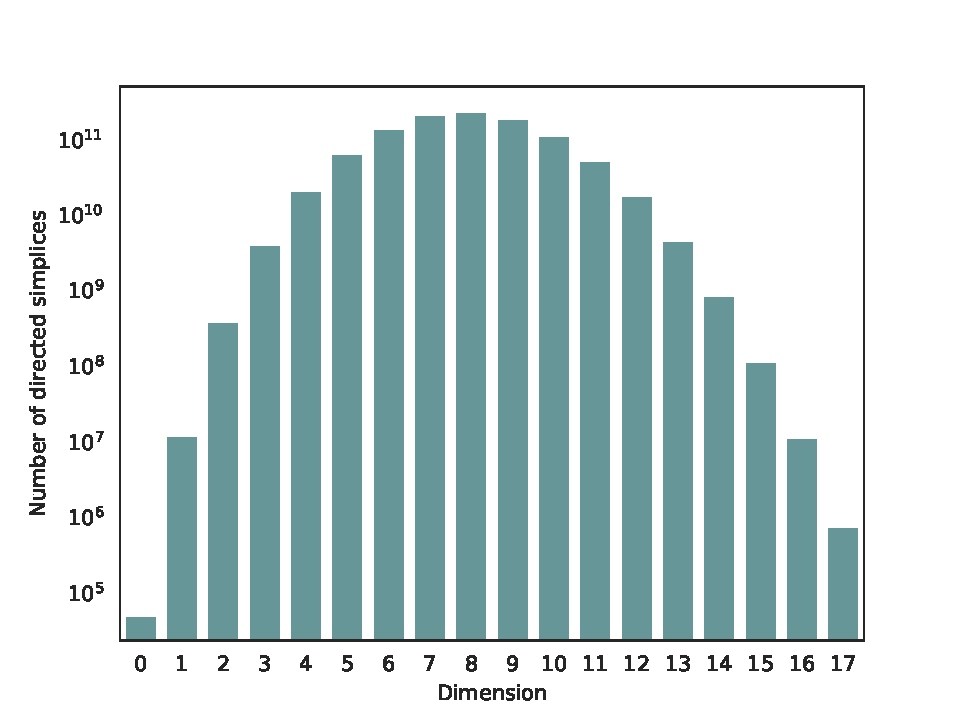
\includegraphics[scale=0.49]{./counts/real50k_count.pdf}
    \caption{ST}
  \end{subfigure}%
  \begin{subfigure}{.49 \linewidth}
    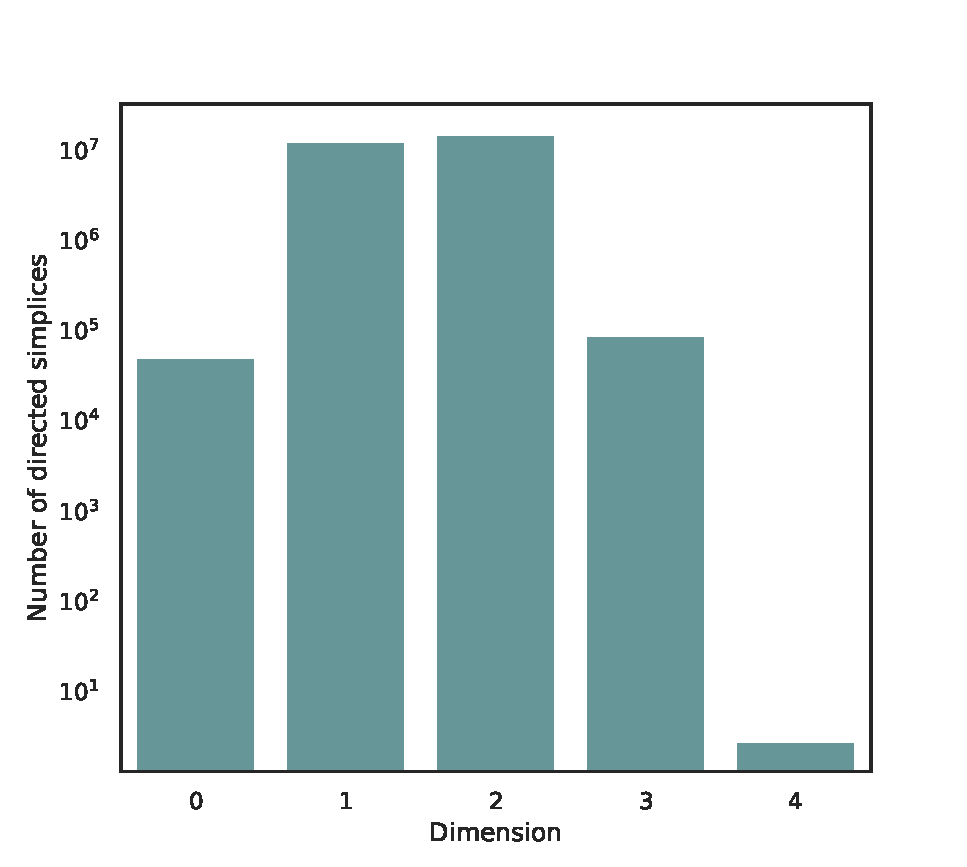
\includegraphics[scale=0.405]{./counts/random50k.pdf}
    \caption{ER}
  \end{subfigure}
  \begin{subfigure}{.45 \linewidth}
    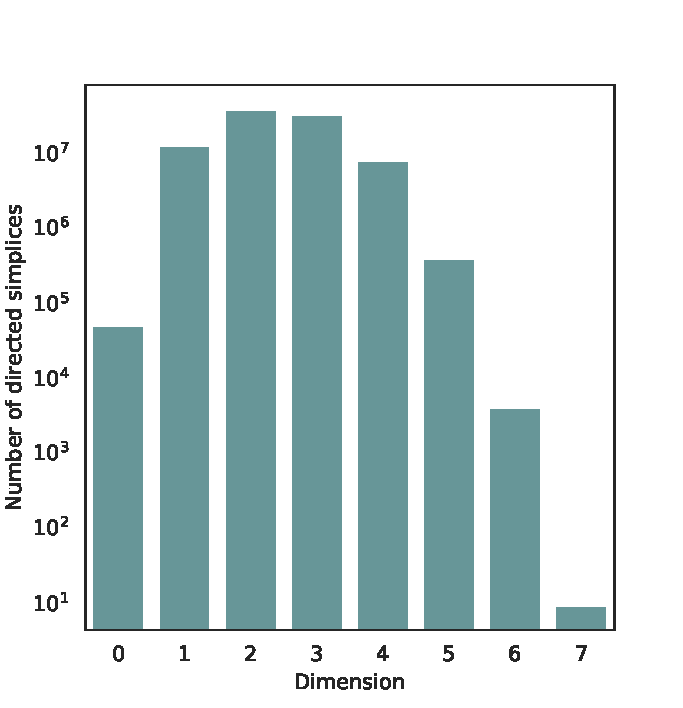
\includegraphics[scale=0.49]{./counts/random50k_ws_count.pdf}
    \caption{WS}
  \end{subfigure}
  \begin{subfigure}{.49 \linewidth}
    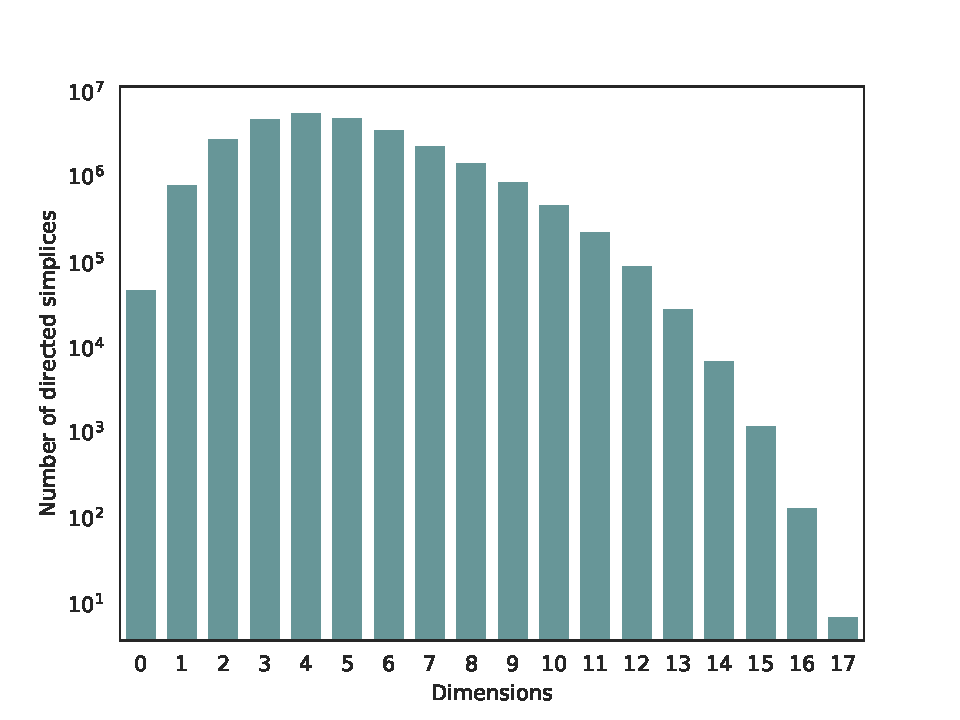
\includegraphics[scale=0.49]{./counts/random50k_ba_count.pdf}
    \caption{BA}
  \end{subfigure}
  \caption{\label{count50k}The total number of simplices in each dimension for the directed flag complex on ST, ER, WS and BA. For ER, WS and BA the counts are the result of the mean number of simplices in each dimension over 100 computations.}
\end{figure}
\begin{table}[ht]
\centering
\begin{tabular}{*4l}    \toprule
  Network & $\beta_{1} $  & $\beta_{2}$  & Computations \\ \toprule
  ST &   $5128 \pm 1219$ & $293013 \pm 79867$ & 1 \\
  ER &  $369770.18 \pm 687.69$ & $3470380.91 \pm 2774.23$ & 100 \\
  WS & $334754.93 \pm 625.38$ & $3756595.22 \pm 3709.97$ & 100 \\
  BA &  $11982.51 \pm 956.18$ & $12946.77  \pm 1734.00$ & 100
  \midrule
  \\
  \bottomrule
\end{tabular}
\caption{\label{bettis} Table over the first and second Betti numbers for the graphs ST, ER, WS and BA. The computation column denotes the number of instances of the model over which the result was averaged, hence the Betti numbers are given by an average value and its standard deviation. For ST the approximation seen in \cite{luetdigraph} was used in order to reduce computational time in which some columns were not reduced to Smith normal form. Every such non-reduced column can at most subtract or add one Betti number.}
\end{table}

\begin{figure}[ht]
  \centering

  \begin{subfigure}{.49 \linewidth}
    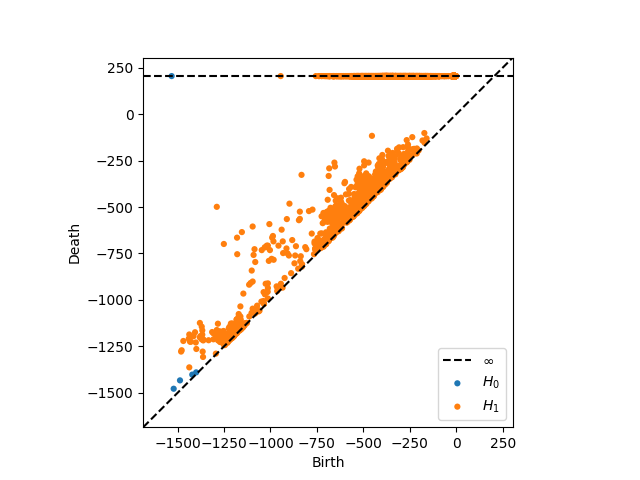
\includegraphics[scale=0.49]{./graph_phs/ST.png}
    \caption{ST}
  \end{subfigure}%
  \begin{subfigure}{.49 \linewidth}
    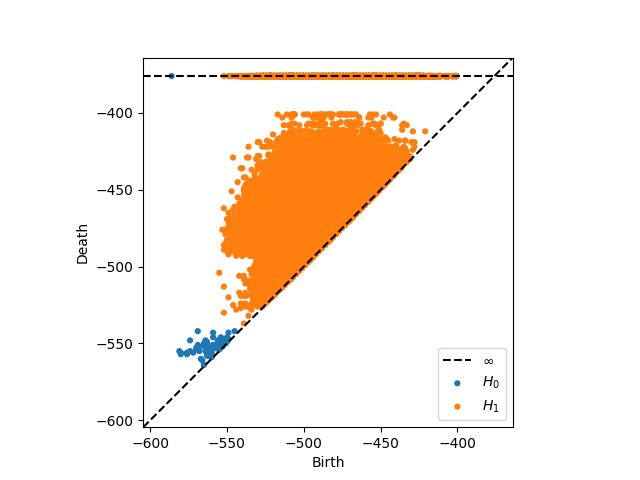
\includegraphics[scale=0.49]{./graph_phs/ER.png}
    \caption{ER}
  \end{subfigure}
  \begin{subfigure}{.49 \linewidth}
    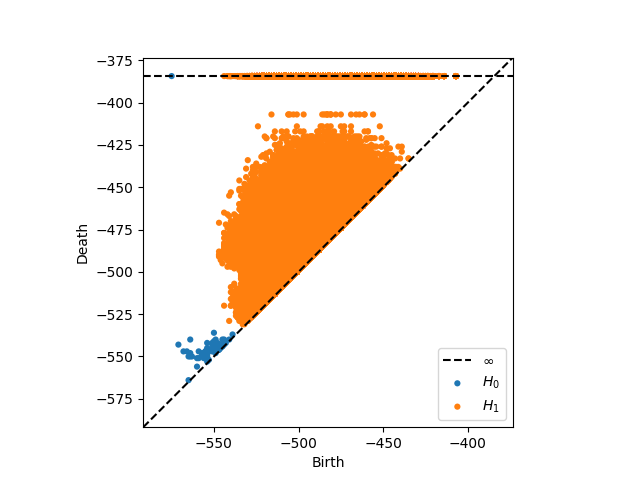
\includegraphics[scale=0.49]{./graph_phs/WG.png}
    \caption{WS}
  \end{subfigure}
  \begin{subfigure}{.49 \linewidth}
    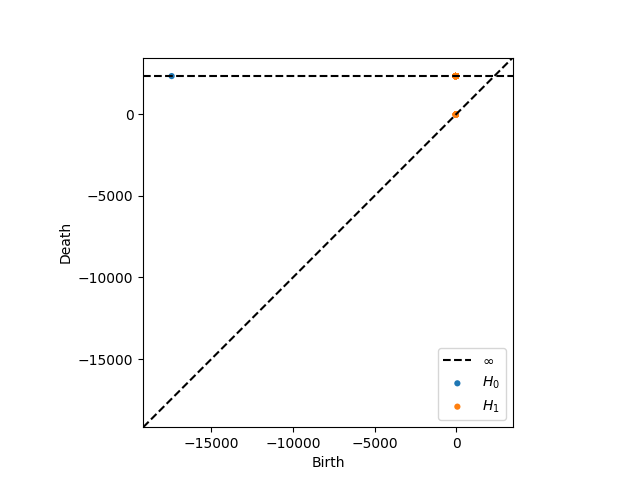
\includegraphics[scale=0.49]{./graph_phs/BA.png}
    \caption{BA}
  \end{subfigure}
  \caption{\label{graphph} Persistence diagrams over $H_{0}$ and $H_{1}$ for ST,ER,WS and BA given by inclusion of vertices and their resulting higher order simplices in the negative order of their degrees.}
\end{figure}

% In Figures \ref{count1k} and \ref{count50k} we see that the synthetic brain networks have much more higher order structure in terms of high dimensional simplices than a network generated solely based on edge connectivity. For instance, we see in \ref{count50k} the presence of 17-dimensional cells in the synthetic network, which means directed cliques consisting of 18 participating neurons, whereas in the random network we see at most 4-dimensional cell.

% In other to further investigate these higher order cells in the synthetic networks we can look at their persistent homology. However, a priori the directed brain network does not have any weights, and so it is not obvious what a filtration $f: V \to \mathbb{R_{+}}$ would look like. So we impose a metric space structure on the directed graph by giving the value of a directed edge between two vertices the Euclidean distance between the two neurons in the simulated model. This means that at low threshold values the filtration will only look at connections made by neurons very close to each other, but as the threshold increases we look at a larger and larger part of the network.

% So what is a generator of a homology group in a brain network? It would have to be a $k$-simplex which is not the boundary of a $k+1$-simplex, which translated to the brain network means a clique of neurons that are in themselves an isolated source-sink network and not part of any other network.

% Due to computational aspects it is not feasible to compute the persistent homology of the synthetic network with 50 001 vertices, so we restrict ourselves to a subnetwork of the full network consisting only of dSPN neurons as seen in Figure \ref{pers50k}. We also look at a full synthetic network generated with only 999 vertices in Figure \ref{pers1k}.

% We see that the formation of higher order $(> 5)$ homology generators mostly happens over small distances, which reaffirms the notion of the brain having a small-world structure.
% \begin{figure}[ht]
%   \centering
%   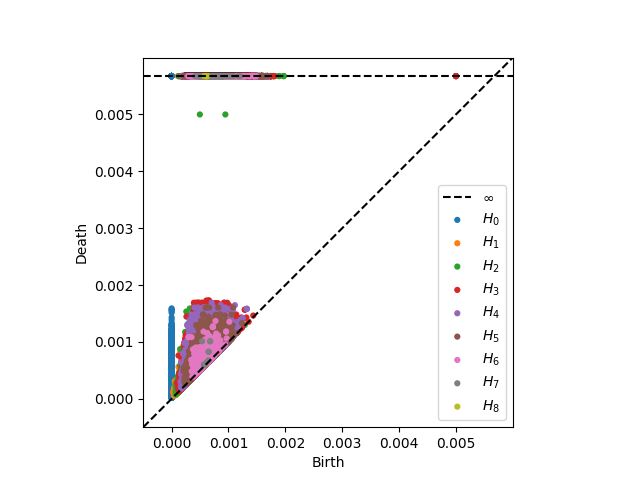
\includegraphics[scale=0.8]{./counts/5kdpsnap10k.png}
%   \caption{\label{pers50k} Persistence diagram of the subnetwork of dSPNs extracted from a synthetic network of 50 001 vertices. }
% \end{figure}

% \begin{figure}[ht]
%   \centering
%   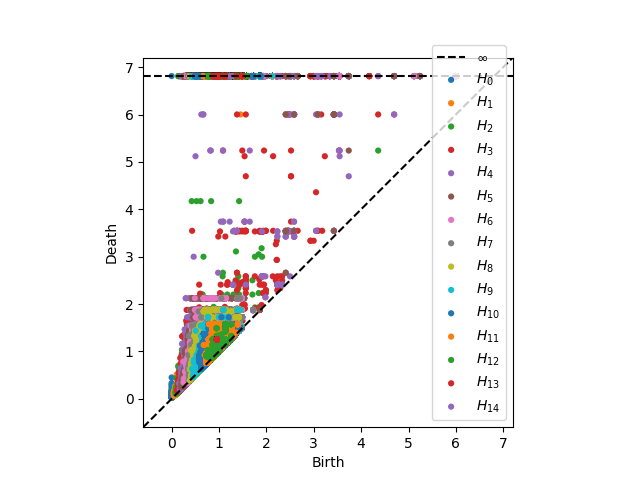
\includegraphics[scale=0.8]{./counts/1kap10000.png}
%   \caption{\label{pers1k} Persistence diagram of the entire synthetic network consisting of 999 vertices. (this is scaled 1000 larger than in actual data, generate new diagram)}
% \end{figure}
%%% Local Variables:
%%% mode: latex
%%% TeX-master: "thesis.tex"
%%% End:

\clearpage
\chapter{Conclusion}


Our goal with this thesis is to provide both an introduction to theory of persistent homology, as well as examples of applications to real-world data. We believe this is  achieved.

We provide an exposition of persistent homology through the concept of a persistence module. We then state and finally prove the unique decomposition of persistence modules into a direct sum of free and torsional parts.  Furthermore, the proof of this theorem yields a concrete algorithm for computing persistent homology of a given filtration. By associating the decomposition with a barcodes, and further on persistence diagrams, we illustrate how persistent homology can be visualized and compared.

On the application side, we present two case studies. These studies are not to be seen as stand-alone results in their respective domains, but rather as examples of how persistent homology can be applied to achieve fruitful insights into data. By using these non-traditional ways of exploring data we hope that we show there is some merit to considering persistent homology as a way of enhancing a traditional data analysis.

In the first case study we analyze 3D scans of the corneas of the bumblebee \textit{Bombus terrestris}. This analysis shows how persistent homology can be applied to volumetric data and how it can be used to perform a clustering and similarity analysis. Furthermore, we are able to find that the persistent homology, specifically the barcode of $H_{2}$ compared across samples with the bottleneck distance, reinforces the already shown hypothesis in \cite{emily}, namely that the morphology of the eyes of \textit{Bombus terrestris} differs between smaller and larger individuals. We also interpret this result as implying that it is the density of the cornea which is a distinguishing factor between differently-sized individuals.

In the second case study we analyze a synthetically generated network made to mimic the micro-circuitry of the striatum. By interpreting the network as a directed graph, we show how persistent homology can be used to compare real-world data given as graphs to control models generated in multiple ways. We reinforce the already established result in \cite{reimann}, that the resulting directed flag complex on the brain network displays a much richer simplicial structure in terms of dimensions and number of simplices compared to control models. Furthermore, we establish that $\beta_{1}$ of the micro-circuitry is much lower than any of the control models. Finally, we see that the distribution of the persistent homology in $H_{1}$ of the micro-circuitry is spread across the entire spectrum of possible degrees, whereas control models only have holes in small intervals of degrees. These observations could act as points of differentiation when it comes to characterizing the striatum.

For some further directions in the first case study, one could extend the methodology to see if $H_{2}$ is always the distinguishing factor within and between different species of insects. However, this would likely require a larger amount of samples.

In the second case study a potential lane of investigation is whether other persistence diagrams of filtrations than the degree based filtration are as unique to the micro-circuitry compared to the other models. Some other filtrations that can be used with the exact same methodology are other measures of importance in a graph, such as the number of shortest path through an edge or the number of neighbors which are neighbors to each other. This is something we wanted to do, but the computational demands together with time restraints made it unfeasible.

Additionally, it could prove fruitful to see whether micro-circuitry in actual the biological striatum displays a similar signature to the synthetic model in terms of persistent homology. Should this be the case, then it strengthens the result of the case study. If it is not the case, then persistent homology could be a parameter to take into account when further calibrating the synthetic model.

%%% Local Variables:
%%% mode: latex
%%% TeX-master: "thesis.tex"
%%% End:

\printbibliography
%\bibliography{thesis}
% TODO:
% Given an equivalence to geometric realization [x]
% Explain compatible bases []
% Make sure that persistence complex is well defined []
% Solve the issue of orientation []
%
%
\end{document}
